\chapter{Result}
\label{ch:intro}

\section{Experimental Environment}

\subsection{Hardware and Software Setup}
All experiments were conducted on a development laptop equipped with an AMD Ryzen™ 7 7735HS processor, 32 GB of DDR5 RAM, and an NVIDIA GPU for accelerated computation , as well as on a \emph{Hunter} mobile robotic platform for on-campus data collection.The robot is equipped with a suite of sensors, including a 3D LiDAR sensor for environment perception, an Inertial Measurement Unit (IMU) for estimating motion and orientation, and a camera for visual reference. An onboard NVIDIA CPU/GPU computing module provides local processing capability.

\begin{figure}[H]
	\centering
	\begin{minipage}{0.5\textwidth}
		\centering
		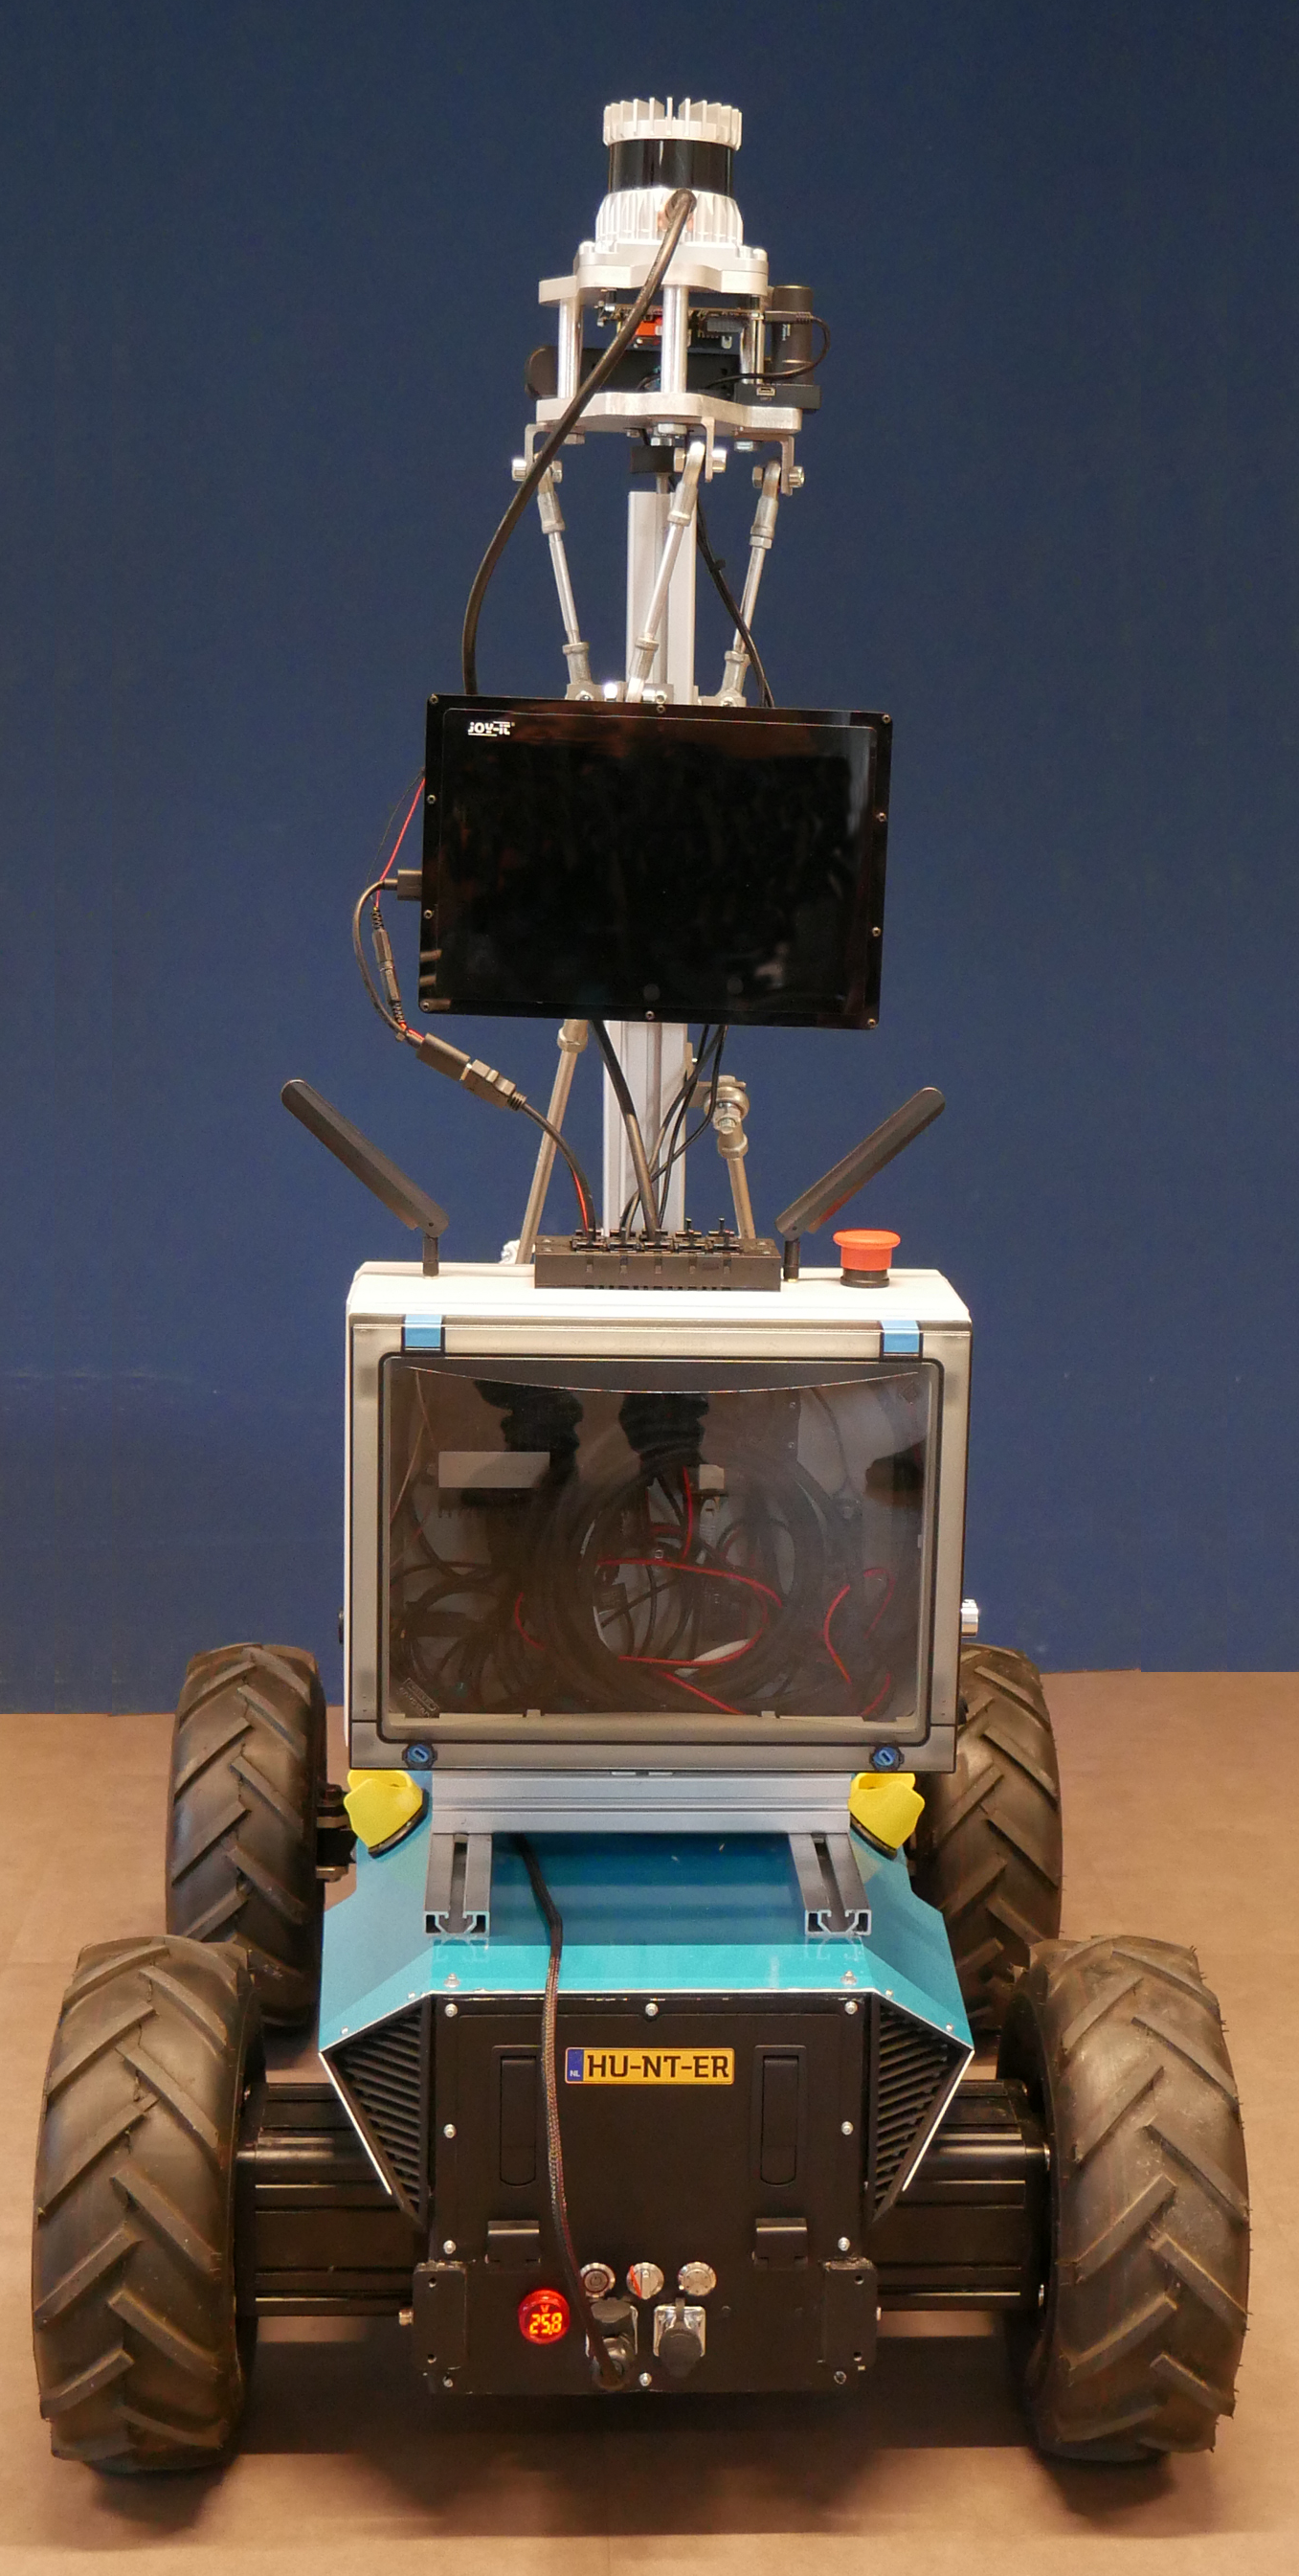
\includegraphics[height=6cm , width=4cm]{images/Hunter_body.png}
		\caption*{(a) Hunter mobile robot platform}
	\end{minipage}\hfill
	\begin{minipage}{0.5\textwidth}
		\centering
		\includegraphics[height=6cm , width=4cm]{images/Hunter_sensor.png}
		\caption*{(b) Sensor configuration (LiDAR, IMU, Camera)}
	\end{minipage}
	\caption{Hardware setup used for real-world data collection and testing: (a) Hunter robotic platform; (b) onboard sensors.}
	\label{fig:hunter-robot-setup}
\end{figure}

Our approach is implemented primarily in C++ on top of the ROS\,2 Humble middleware. We rely on:
\begin{itemize}
  \item \textbf{PCL (Point Cloud Library):} for point cloud data structures and filtering.
  \item \textbf{Eigen:} for linear algebra operations (transformations, matrix computations).

\end{itemize}
Additional scripts in Python were employed for plotting and minor data manipulations.

\subsection{Datasets and Map Preparation}
We evaluated our map-based localization on multiple datasets, each of which offers LiDAR and IMU data. Table~\ref{tab:datasets} summarizes their key characteristics.

\begin{table}[htbp]
	\centering
	\caption{Overview of datasets and sensor configurations. (L: LiDAR; I: IMU)}
	\label{tab:datasets}
	\resizebox{\textwidth}{!}{%
	\begin{tabular}{lccccc}
	\toprule
	\textbf{Dataset} & \textbf{Seq.} & \textbf{Sensors} & \textbf{LiDAR Type} & \textbf{Frequencies (Hz)} & \textbf{Map Prep. Method} \\
	\midrule
	\textbf{KITTI Odometry} & 05 & L + I & Velodyne HDL-64E & L: 10, I: 100 & GT-based aggregation \\
	%\textbf{KITTI Odometry} & 09 & L + I & Velodyne HDL-64E & L: 10, I: 100 & GT-based aggregation \\
	\textbf{MulRan}         & KiAST-02,03 & L + I & Ouster OS1-64    & L: 10, I: 100 & Fast-LIO2 SLAM \\
	\textbf{Saxion Dataset}  & seq1,2,3 & L + I & Ouster OS1-128    & L: 10, I: 100 & Fast-LIO2 SLAM \\
	
	\bottomrule
	\end{tabular}%
	}
\end{table}



\paragraph{Benchmark Dataset}
 We used sequences 05 from the KITTI odometry benchmark\cite{Geiger2012KITTI} and two sequences (KiAST-02, KiAST-03) from the MulRan dataset\cite{Kim2020Mulran},both representing semi-urban driving scenarios with moderate speeds.The official ground-truth poses were used to transform and aggregate each LiDAR frame into a global coordinate system for generate 3D priori map.
\paragraph{Custom Saxion Dataset}
 As no direct ground truth was available for this dataset, we employed Fast-LIO2 SLAM to generate a consistent map from repeated traversals. 

In both cases, the final global point cloud is subdivided into manageable tiles for efficient local map loading during localization. Each tile is stored as a separate file or database entry keyed by tile coordinates, allowing the system to load only relevant tiles based on the vehicle’s current estimated position.


\section{Performance Evaluation}
This section presents the experimental results evaluating the proposed LiDAR-inertial localization system. The evaluation is divided into two main parts: performance under standard conditions, and extended experiments conducted under different scenarios to assess system robustness. Standard conditions refer to scenario where the reference map is up-to-date, sensor data is relatively noise-free, and feature-rich map. In contrast, under extended scenarios, we test robustness by replaying the same trajectory through map transition zones, with composite geometric noise (simulating fog, rain, and snow), slight map aging, and dynamic object removal.

Overall, we evaluate localization performance in terms of Absolute Pose Error (APE), convergence behavior, and real-time processing latency. The evaluation includes comparisons against two categories of baselines: component baselines, which consist of the individual modules integrated into our system (Fast-LIO2\cite{xuFastLIO2} and NDT\cite{biber2003ndt} scan matching), and external SLAM baselines, such as MOLA\cite{blanco2025mola_lo} and KISS-SLAM\cite{kiss2025arxiv}, which represent complete state estimation frameworks used for comparative benchmarking.

\subsection{ Localization Performance in Standard Conditions}

\subsubsection{Saxion Campus Dataset}
We evaluated our proposed LiDAR-inertial localization system on three sequences collected from the Saxion campus, representing short, medium, and long trajectories with varying coverage areas and trajectory complexity.Quantitative performance is assessed using Absolute Pose Error (APE) and rotational error after SE(3) alignment.

 Table \ref{tab:ape_rot_saxion_seq1} , \ref{tab:ape_rot_saxion_seq2} , \ref{tab:ape_rot_saxion_seq3} summarize translation and rotation error statistics, including maximum, mean, and RMSE values for the three Saxion sequences. The results show that the proposed fusion-based system consistently outperforms both baseline methods across all sequences. In Sequence 1, the proposed method achieves centimeter-level accuracy, with  translation RMSE of 0.067 m, which is approximately 33× lower than the RMSE of 2.197 m observed with Fast-LIO2. The rotational RMSE is also reduced from 2.072° to 0.583°, indicating significant drift correction not only in position but also in orientation.

 In the longer and more complex trajectories (Sequences 2 and 3), the proposed fusion method achieves decimeter-level accuracy, significantly reducing translational RMSE compared to Fast-LIO2 (from 3.3 m to 0.11–0.13 m) and improving rotational RMSE by up to 1.6°. While NDT achieves similar translational RMSE in some cases, the fusion method offers better rotational accuracy and stability, especially under challenging conditions.
 
Trajectory plots Figures \ref{fig:saxion-seq1-trajectory-zoom}~ \ref{fig:saxion-seq2-trajectory-zoom}~\ref{fig:saxion-seq3-trajectory-zoom}  illustrate the alignment of estimated poses with reference trajectory. Zoomed-in regions further emphasize the proposed method’s ability to track the trajectory accurately, even in complex zones and long trajectory.



\begin{table}[H]
	\centering
	\renewcommand{\arraystretch}{0.6}
	\setlength{\tabcolsep}{15pt}
	\caption{Translation (APE) and Rotation Error statistics for Saxion \textbf{Sequence 1} }
	\captionsetup{justification=justified, singlelinecheck=false}
	
	
	\label{tab:ape_rot_saxion_seq1}
	
	\begin{adjustbox}{width=\textwidth}
		\begin{tabular}{@{}lccccccc@{}}
			\toprule
			\textbf{Method} & \textbf{Metric} & \textbf{Max} & \textbf{Mean} & \textbf{Median} & \textbf{Min} & \textbf{RMSE} & \textbf{Std Dev} \\
			\midrule
			
			\multirow{2}{*}{\textbf{Proposed (Fusion)}} 
			& APE (m)        & 0.395   & \textbf{0.052 }   & \textbf{0.041}     & \textbf{0.003 }   &\textbf{ 0.067}   & \textbf{0.042 }\\
			& Rot. (deg)     & \textbf{4.715}   & \textbf{0.321}    & \textbf{0.169}     &\textbf{ 0.030 }   & \textbf{0.583}   &\textbf{ 0.486} \\
			\midrule
			
			\multirow{2}{*}{NDT Scan Matching} 
			& APE (m)        & \textbf{0.363 }  & 0.074    & 0.067     & 0.012    & 0.084   & \textbf{0.041} \\
			& Rot. (deg)     & 5.832   & 0.503    & 0.299     &\textbf{ 0.012}    & 0.813   & 0.639 \\
			\midrule
			
			\multirow{2}{*}{Fast-LIO2} 
			& APE (m)        & 7.594   & 1.456    & 0.933     & 0.322    & 2.197   & 1.645 \\
			& Rot. (deg)     & 6.213   & 1.631    & 1.304     & 0.419    & 2.072   & 1.278 \\
			\bottomrule
		\end{tabular}
	\end{adjustbox}
\vspace{0.5em}
{\footnotesize \textit{Note:} Bold values indicate the best performance across each metric.}
\end{table}

\begin{figure}[H]
	\centering
	\begin{tikzpicture}
		% Main trajectory image
		\node[anchor=south west, inner sep=0] (main) at (0,0)
		{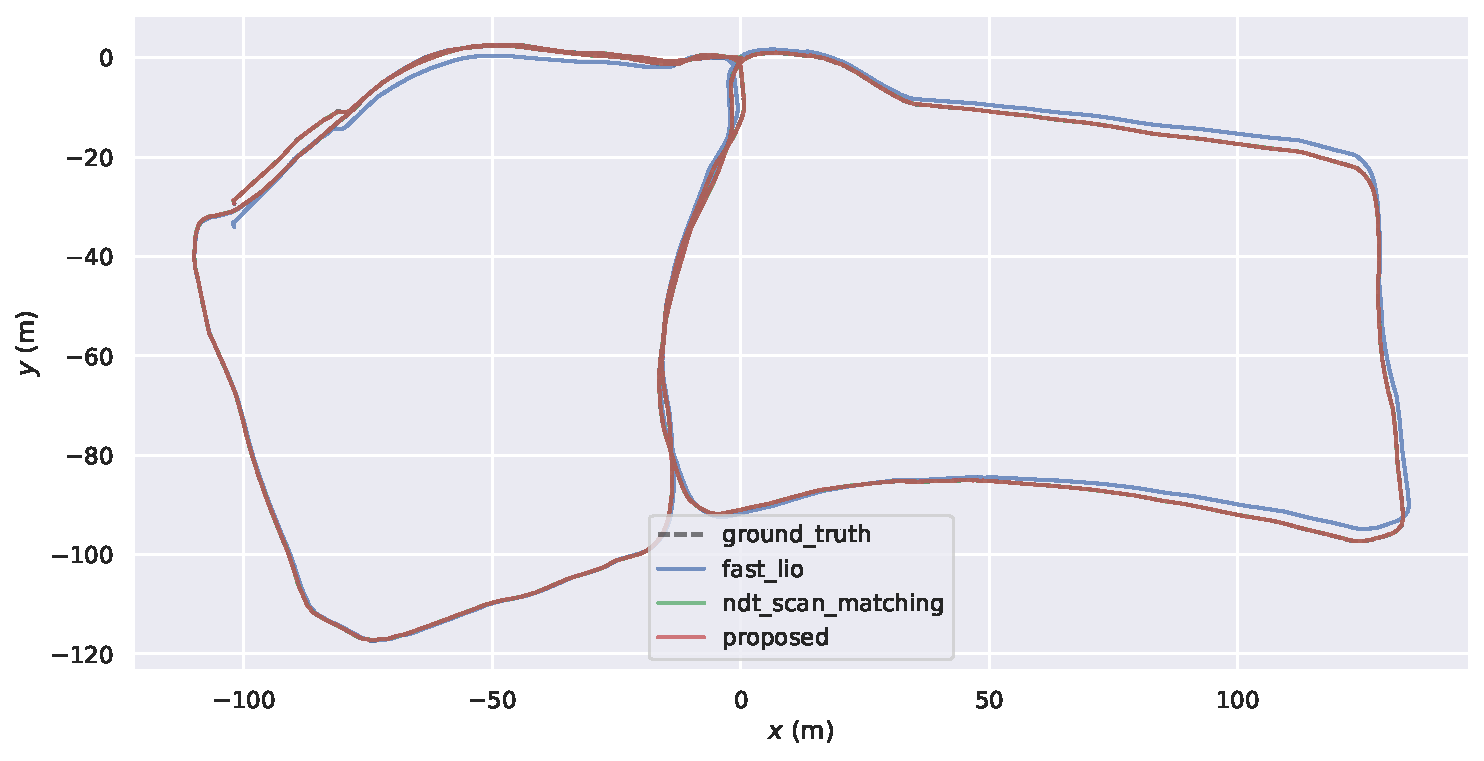
\includegraphics[page=1 , width=0.8\textwidth]{images/trajectory_plot_seq1.pdf}};
		% Coordinate system normalized to the image
		\begin{scope}[x={(main.south east)}, y={(main.north west)}]
			% Red dashed rectangle for zoom box (adjust coordinates!)
			\draw[red, thick, dashed] (0.85, 0.20) rectangle (0.98, 0.45);
			% Red arrow from zoom box to zoomed-in image
			\draw[->, red, thick] (0.98, 0.45) -- (1, 0.85);
		\end{scope}
		% Zoomed-in image overlay (use exact x/y in cm to place)
		\node[anchor=south west] at (8, 6)
		{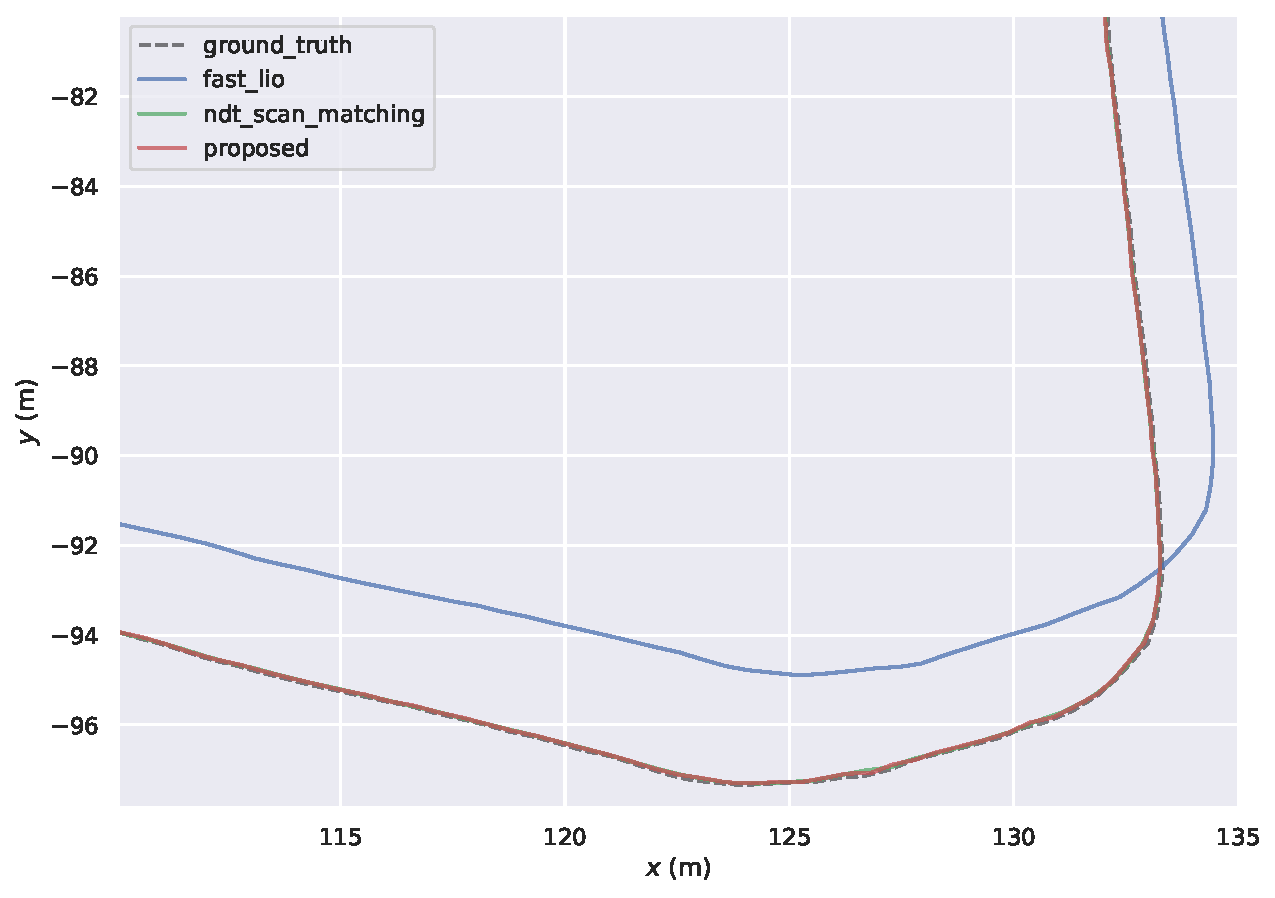
\includegraphics[width=0.5\textwidth]{images/trajectory_zoom_seq1.pdf}};
		% Optional label
		%\node at (15, 4.6) {\small Zoomed-in detail};
	\end{tikzpicture}
	\caption[Saxion Sequence 01 – Trajectory Alignment with Zoomed Comparison]%
	{\textbf{Saxion Sequence 01 – Trajectory Alignment.} 
		The figure shows the estimated trajectories from FAST-LIO2, low frequency NDT map matching , and the proposed method, overlaid against ground truth. The red dashed box indicates the zoomed region.
	}
	\label{fig:saxion-seq1-trajectory-zoom}
\end{figure}


\begin{table}[H]
	\centering
	\renewcommand{\arraystretch}{0.6}
	\setlength{\tabcolsep}{15pt}
	\caption{Translation (APE) and Rotation Error statistics for Saxion \textbf{Sequence 2} }
	\label{tab:ape_rot_saxion_seq2}
	
	\begin{adjustbox}{width=\textwidth}
		\begin{tabular}{@{}lccccccc@{}}
			\toprule
			\textbf{Method} & \textbf{Metric} & \textbf{Max} & \textbf{Mean} & \textbf{Median} & \textbf{Min} & \textbf{RMSE} & \textbf{Std Dev} \\
			\midrule
			
			\multirow{2}{*}{\textbf{Proposed (Fusion)}} 
			& APE (m)        & 0.440   & \textbf{0.090}   & \textbf{0.075}     & \textbf{0.005}   & \textbf{0.107}   & \textbf{0.058} \\
			& Rot. (deg)     & 4.356   & \textbf{0.782}   & \textbf{0.539}     & \textbf{0.051}   & \textbf{1.046}   & \textbf{0.695} \\
			\midrule
			
			\multirow{2}{*}{NDT Scan Matching} 
			& APE (m)        & \textbf{0.245}   & 0.102   & 0.094     & 0.009    & 0.118   & 0.059 \\
			& Rot. (deg)     & \textbf{2.639}   & 1.195   & 1.127     & 0.103    & 1.393   & 0.715 \\
			\midrule
			
			\multirow{2}{*}{Fast-LIO2} 
			& APE (m)        & 9.467   & 2.507   & 1.944     & 0.370    & 3.301   & 2.147 \\
			& Rot. (deg)     & 5.494   & 2.250   & 1.568     & 0.202    & 2.680   & 1.456 \\
			\bottomrule
		\end{tabular}
	\end{adjustbox}

\vspace{0.5em}
{\footnotesize \textit{Note:} Bold values indicate the best performance across each metric.}
\end{table}


\begin{table}[H]
	\centering
	\renewcommand{\arraystretch}{0.6}
	\setlength{\tabcolsep}{15pt}
	\caption{Translation (APE) and Rotation Error statistics for Saxion \textbf{Sequence 3} }
	\label{tab:ape_rot_saxion_seq3}
	
	\begin{adjustbox}{width=\textwidth}
		\begin{tabular}{@{}lccccccc@{}}
			\toprule
			\textbf{Method} & \textbf{Metric} & \textbf{Max} & \textbf{Mean} & \textbf{Median} & \textbf{Min} & \textbf{RMSE} & \textbf{Std Dev} \\
			\midrule
			
			\multirow{2}{*}{\textbf{Proposed (Fusion)}} 
			& APE (m)        & 0.821   & \textbf{0.097}   & \textbf{0.072}     & \textbf{0.004}   & 0.135   & 0.094 \\
			& Rot. (deg)     & 5.016   & \textbf{0.725}   & \textbf{0.472}     & \textbf{0.076}   & \textbf{1.039}   & \textbf{0.743} \\
			\midrule
			
			\multirow{2}{*}{NDT Scan Matching} 
			& APE (m)        & \textbf{0.297}   & 0.113   & 0.100     & 0.025    & \textbf{0.126}   & \textbf{0.056} \\
			& Rot. (deg)     & 3.236   & 1.373   & 1.286     & 0.131    & 1.652   & 0.919 \\
			\midrule
			
			\multirow{2}{*}{Fast-LIO2} 
			& APE (m)        & 3.475   & 1.468   & 1.254     & 0.028    & 1.862   & 1.145 \\
			& Rot. (deg)     & 2.750   & 0.955   & 0.953     & 0.069    & 1.088   & 0.522 \\
			\bottomrule
		\end{tabular}
	\end{adjustbox}
{\footnotesize \textit{Note:} Bold values indicate the best performance across each metric.}
\end{table}



\subsubsection{Comparison with SLAM Methods }

To benchmark the proposed system against existing SLAM methods, we evaluated it on KITTI Sequence 05, which includes multiple natural loop closures alongside KISS-ICP  and MOLA SLAM. As shown in Table~\ref{tab:ape_rot_kitti_seq5}, the proposed method achieves significantly lower translation and rotation errors, attaining decimeter-level accuracy through the incorporation of map-based scan matching and factor-graph fusion.

Despite the presence of loop closures, both SLAM methods exhibit notable drift and large maximum errors with translational APE reaching up to 6.8\,m and rotational errors exceeding {3.8°}. These results underline a key limitation of SLAM: its reliance on successful and timely loop closure events to correct long-term drift. In contrast, the proposed approach leverages a prebuilt map to maintain global consistency at all times, avoiding error accumulation. As visualized in Figure~\ref{fig:kitti05-traj-zoom}, the proposed trajectory remains well-aligned with the reference path throughout the sequence, while SLAM methods show clear deviation, especially toward the end. This demonstrates the robustness and reliability of map-based localization  even under conditions favorable to SLAM.

\begin{table}[H]
	\centering
	\renewcommand{\arraystretch}{0.6}
	\setlength{\tabcolsep}{15pt}
	\caption{Translation (APE) and Rotation Error statistics for \textbf{KITTI Sequence 05}}
	\label{tab:ape_rot_kitti_seq5}
	
	\begin{adjustbox}{width=\textwidth}
		\begin{tabular}{@{}lccccccc@{}}
			\toprule
			\textbf{Method} & \textbf{Metric} & \textbf{Max} & \textbf{Mean} & \textbf{Median} & \textbf{Min} & \textbf{RMSE} & \textbf{Std Dev} \\
			\midrule
			
			\multirow{2}{*}{\textbf{Proposed}} 
			& APE (m)        & \textbf{0.483}   & \textbf{0.121}   & \textbf{0.102}     & \textbf{0.007}   & \textbf{0.143}   & \textbf{0.077} \\
			& Rot. (deg)     & \textbf{1.914}   & \textbf{0.376}   & \textbf{0.356}     & \textbf{0.078}   & \textbf{0.402}   & \textbf{0.144} \\
			\midrule
			
			\multirow{2}{*}{KISS-ICP} 
			& APE (m)        & 5.067   & 1.460   & 1.445     & 0.281    & 1.604   & 0.666 \\
			& Rot. (deg)     & 2.696   & 1.376   & 1.441     & 0.000    & 1.465   & 0.504 \\
			\midrule
			
			\multirow{2}{*}{MOLA SLAM} 
			& APE (m)        & 6.817   & 1.539   & 1.447     & 0.306    & 1.793   & 0.920 \\
			& Rot. (deg)     & 3.861   & 1.931   & 1.886     & 0.000    & 2.015   & 0.577 \\
			\bottomrule
		\end{tabular}
	\end{adjustbox}

{\footnotesize \textit{Note:} Bold values indicate the best performance across each metric.}
\end{table}


\begin{figure}[H]
	\centering
	\begin{tikzpicture}
		
		% Main trajectory image
		\node[anchor=south west, inner sep=0] (main) at (0,0)
		{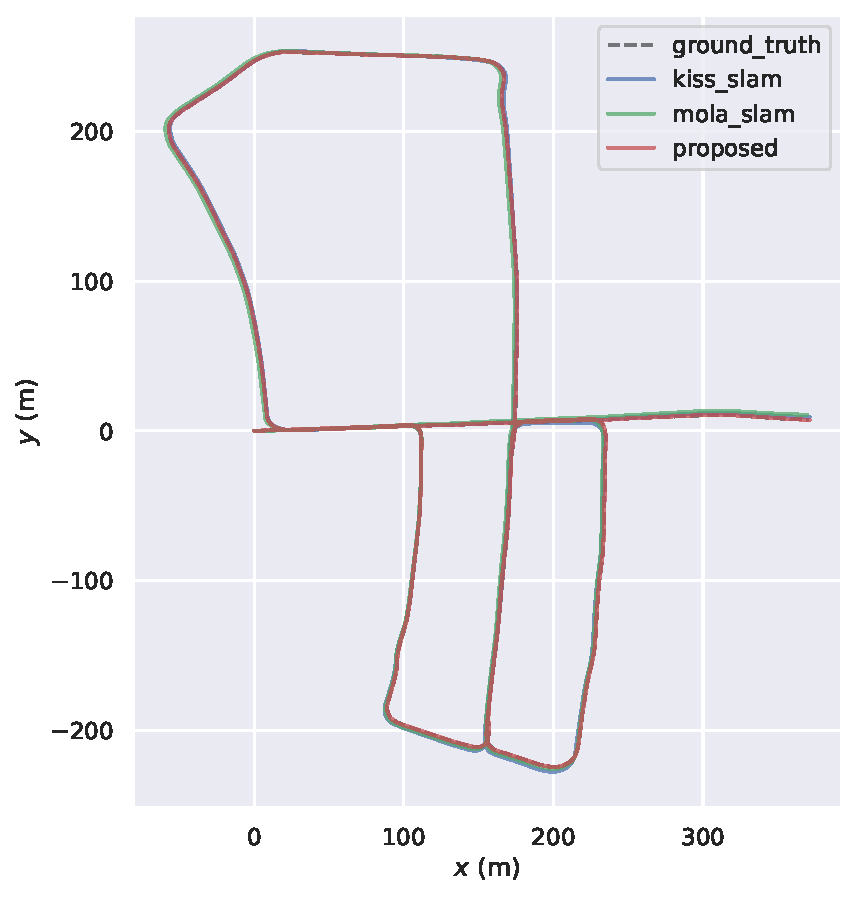
\includegraphics[width=0.75\textwidth]{images/trajectory_plot_kitti.pdf}};
		% Coordinate system normalized to the image
		\begin{scope}[x={(main.south east)}, y={(main.north west)}]
			% Red dashed rectangle for zoom box (adjust coordinates!)
			\draw[red, thick, dashed] (0.85, 0.5) rectangle (0.95, 0.56);
			% Red arrow from zoom box o tzoomed-in image
			\draw[->, red, thick] (0.95, 0.55) -- (0.97, 0.57);
		\end{scope}
		
		% Zoomed-in image overlay (use exact x/y in cm to place)
		\node[anchor=south west] at (8.1, 7.2)
		{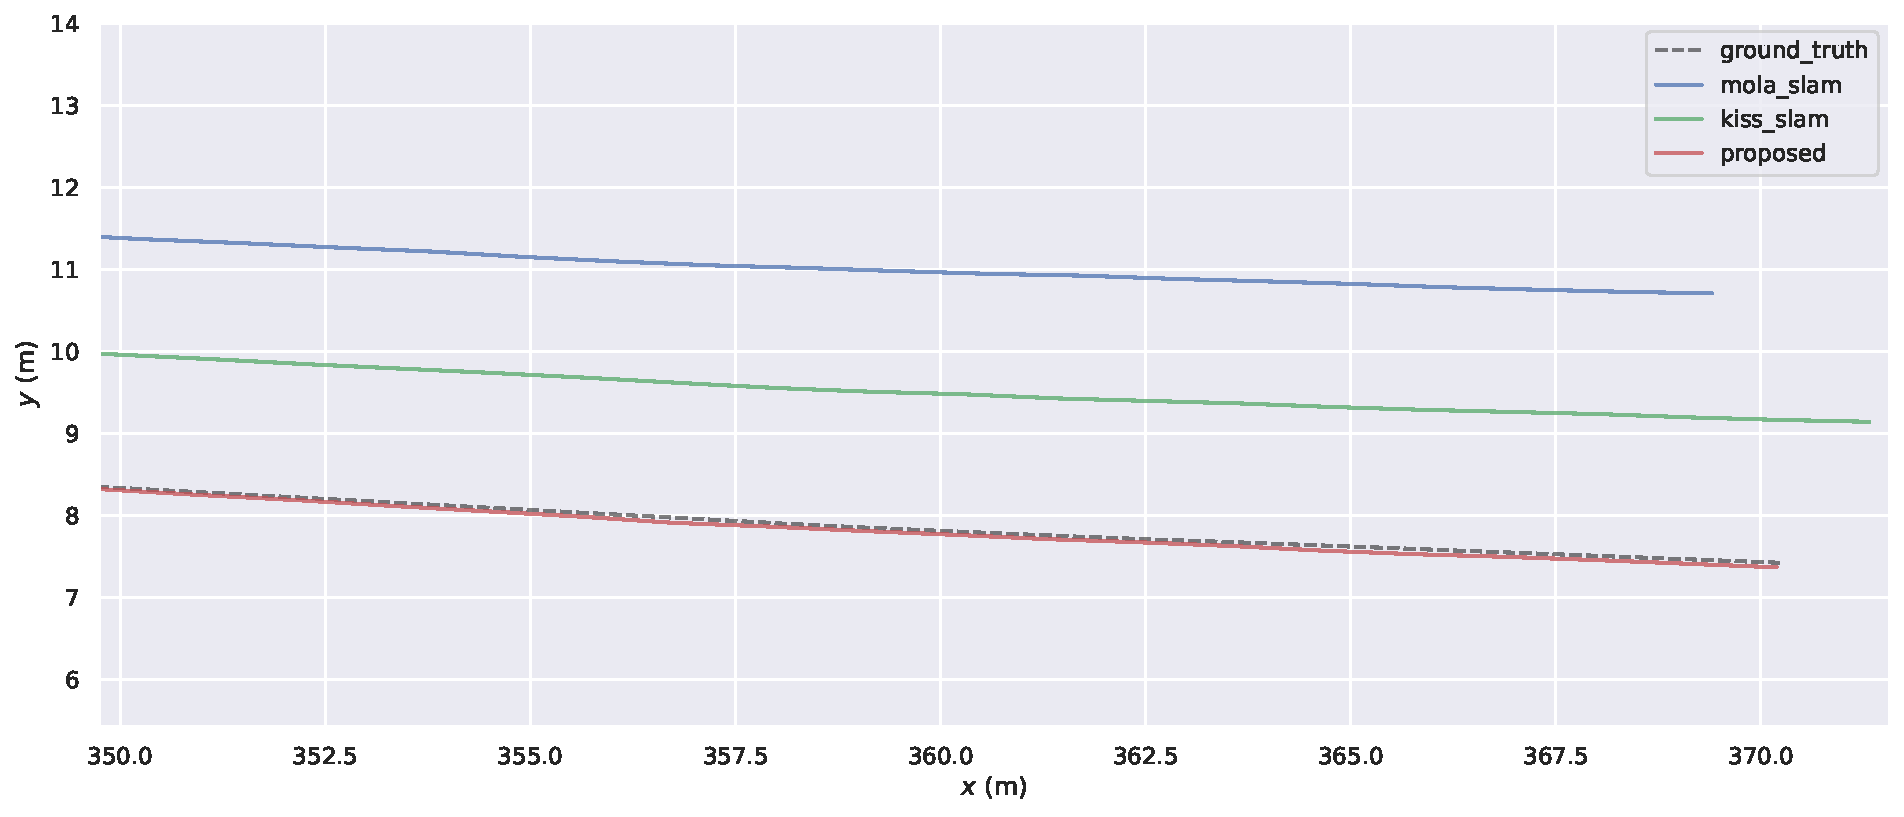
\includegraphics[width=0.45\textwidth]{images/trajectory_plot_kitti_zoom.pdf}};
		
		% Optional label
		%\node at (15, 4.6) {\small Zoomed-in detail};
		
	\end{tikzpicture}
	
	\caption[KITTI Sequence 05 – Trajectory Alignment with Zoomed Comparison]%
	{\textbf{KITTI Sequence 05 – Trajectory Alignment.} 
		The figure shows the estimated trajectories from KISS-SLAM, MOLA SLAM, and the proposed method, overlaid against ground truth.The red dashed box indicates the zoomed region..
	}
	\label{fig:kitti05-traj-zoom}
\end{figure}

\subsubsection{Real-time Performance }

We evaluate  scan-to-map matching by varying the radius of the local sub map and compare multi-threaded
NDT (NDT-OMP) , standard NDT and classic ICP all operating on identically generated local maps.As shown in the table \ref{tab:scanmap_radius} While both NDT and ICP maintain convergence on small radii (> 100 m), their per‐scan runtime  is exceed 100 ms and increases as map grows.In contrast, NDT-OMP maintains sub-25 ms mean latency with over 95 $\%$ convergence up to 200 m, and still achieves under 33 ms runtimes and 90 $\%$ convergence at 350 m (with occasional failures). This demonstrates that NDT-OMP’s parallelization, coupled with an adaptive local-map radius based on the robot’s pose, significantly improves scan-matching efficiency without sacrificing robustness.



\begin{table}[H]
	\centering
	\caption{Scan‐Matching Performance vs.\ Local Map Radius}
	\renewcommand{\arraystretch}{0.5}
	\setlength{\tabcolsep}{1pt}
	\label{tab:scanmap_radius}
	\begin{tabular}{c l c c c}
		\toprule
		\textbf{Map Radius(m)} & \textbf{Method} & \textbf{Mean Time(ms)} & \textbf{Converged(\%)} & \textbf{Remarks} \\
		\midrule
		100 & NDT     & 90  & 90 &  \\
		& ICP     & >100  & 90 &             \\
		& NDT‐OMP(8 thread) &  15  & 99 &     \\
			\midrule
		\addlinespace
		200 & NDT     & >100  & <50 &  failures           \\
		& ICP     & >100  & <50&       failures     \\
		& NDT‐OMP(8 thread) & 20  & 97 &            \\
			\midrule
		\addlinespace
		350 & NDT     & >100  & <50 &  failures \\
		& ICP     & >100 &     <50 &  failures          \\
		& NDT‐OMP(8 thread) & 25  & 90 &  some failures     \\
		\bottomrule
	\end{tabular}
\end{table}

\begin{figure}[H]
	\centering
	\begin{subfigure}[t]{0.48\textwidth}
		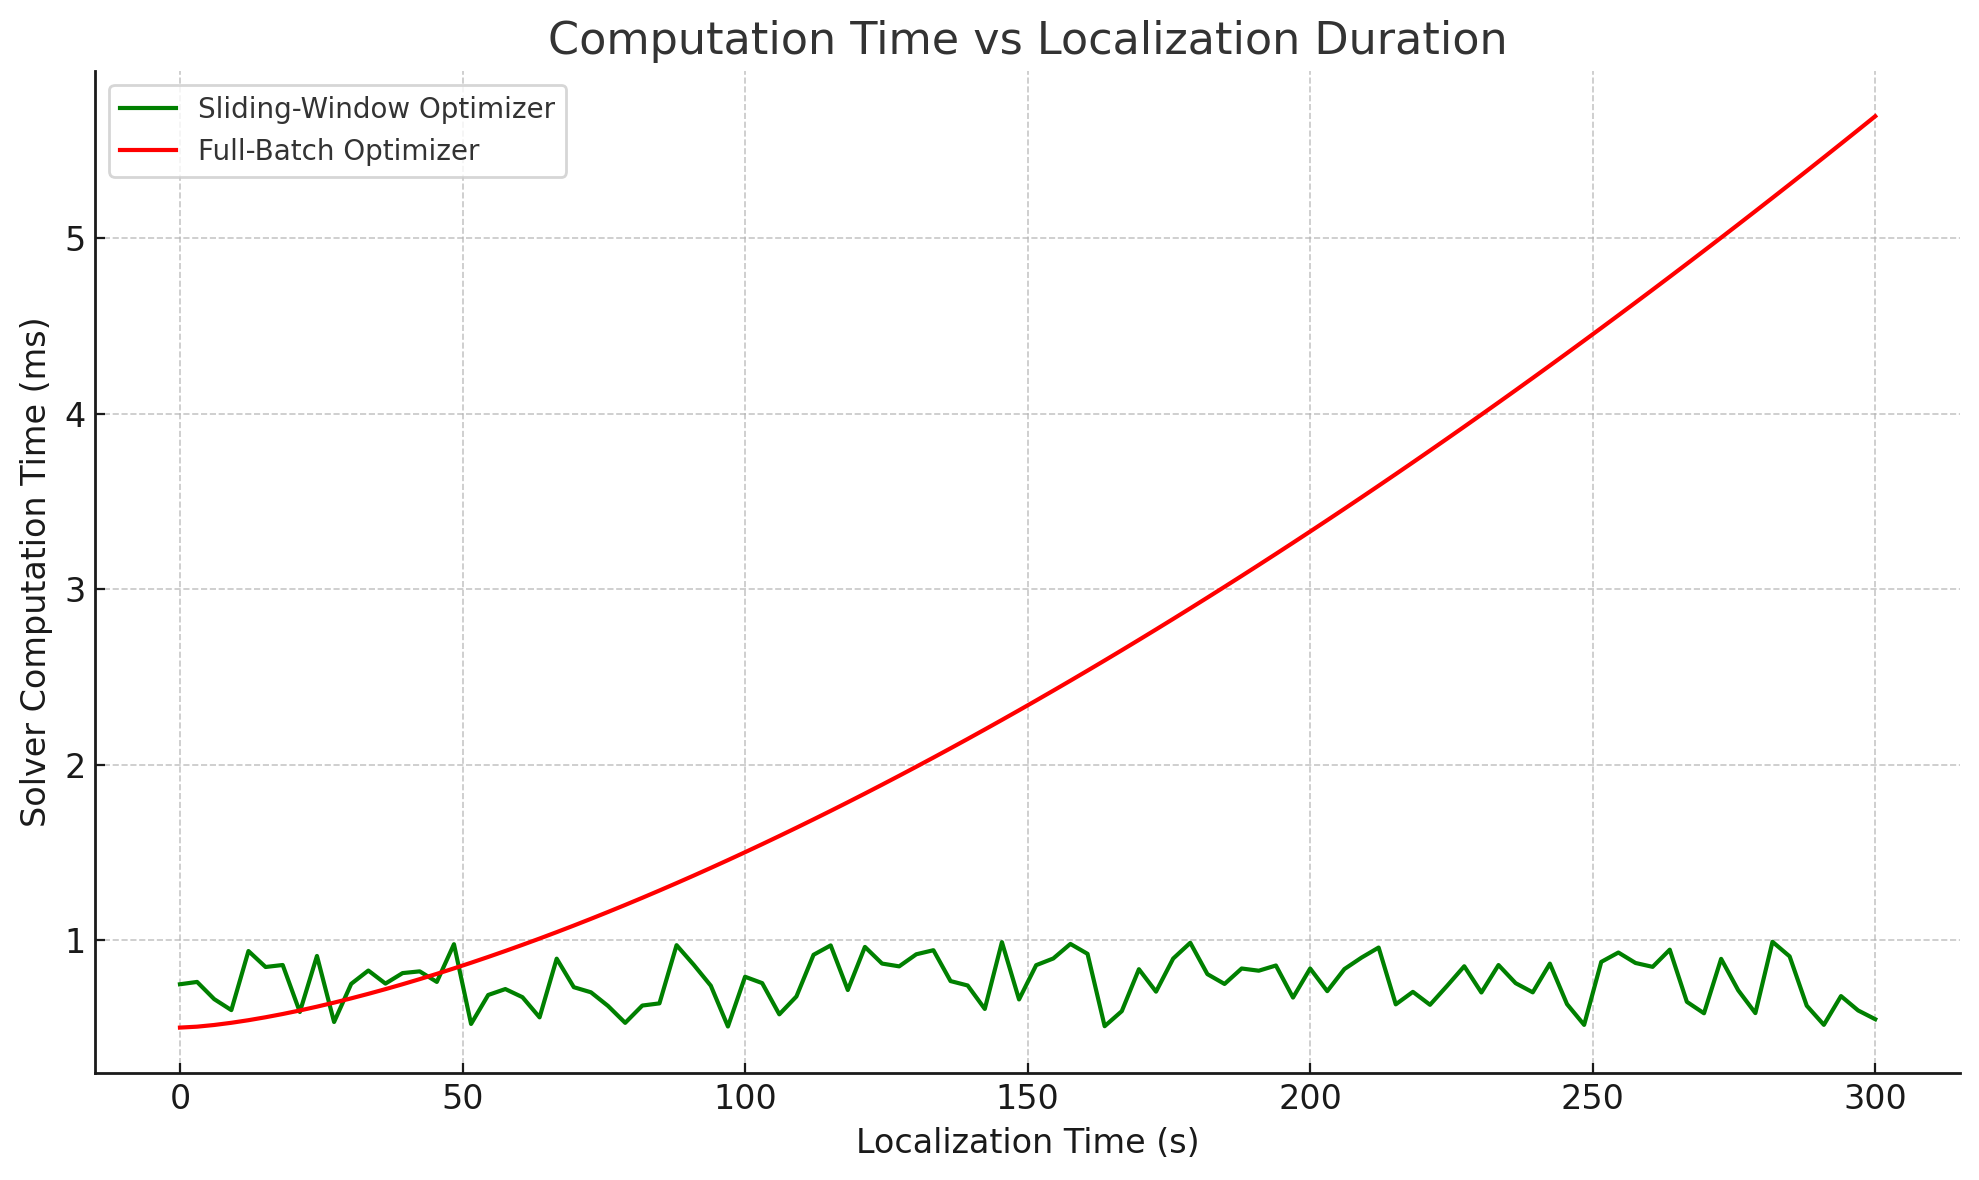
\includegraphics[ width=\linewidth , height=\linewidth]{images/compration_registration_alg.png}
		\caption{Computation time trend of sliding-window vs full-batch optimizer.}
		\label{fig:sliding_vs_batch}
	\end{subfigure}
	\hfill
	\begin{subfigure}[t]{0.48\textwidth}
		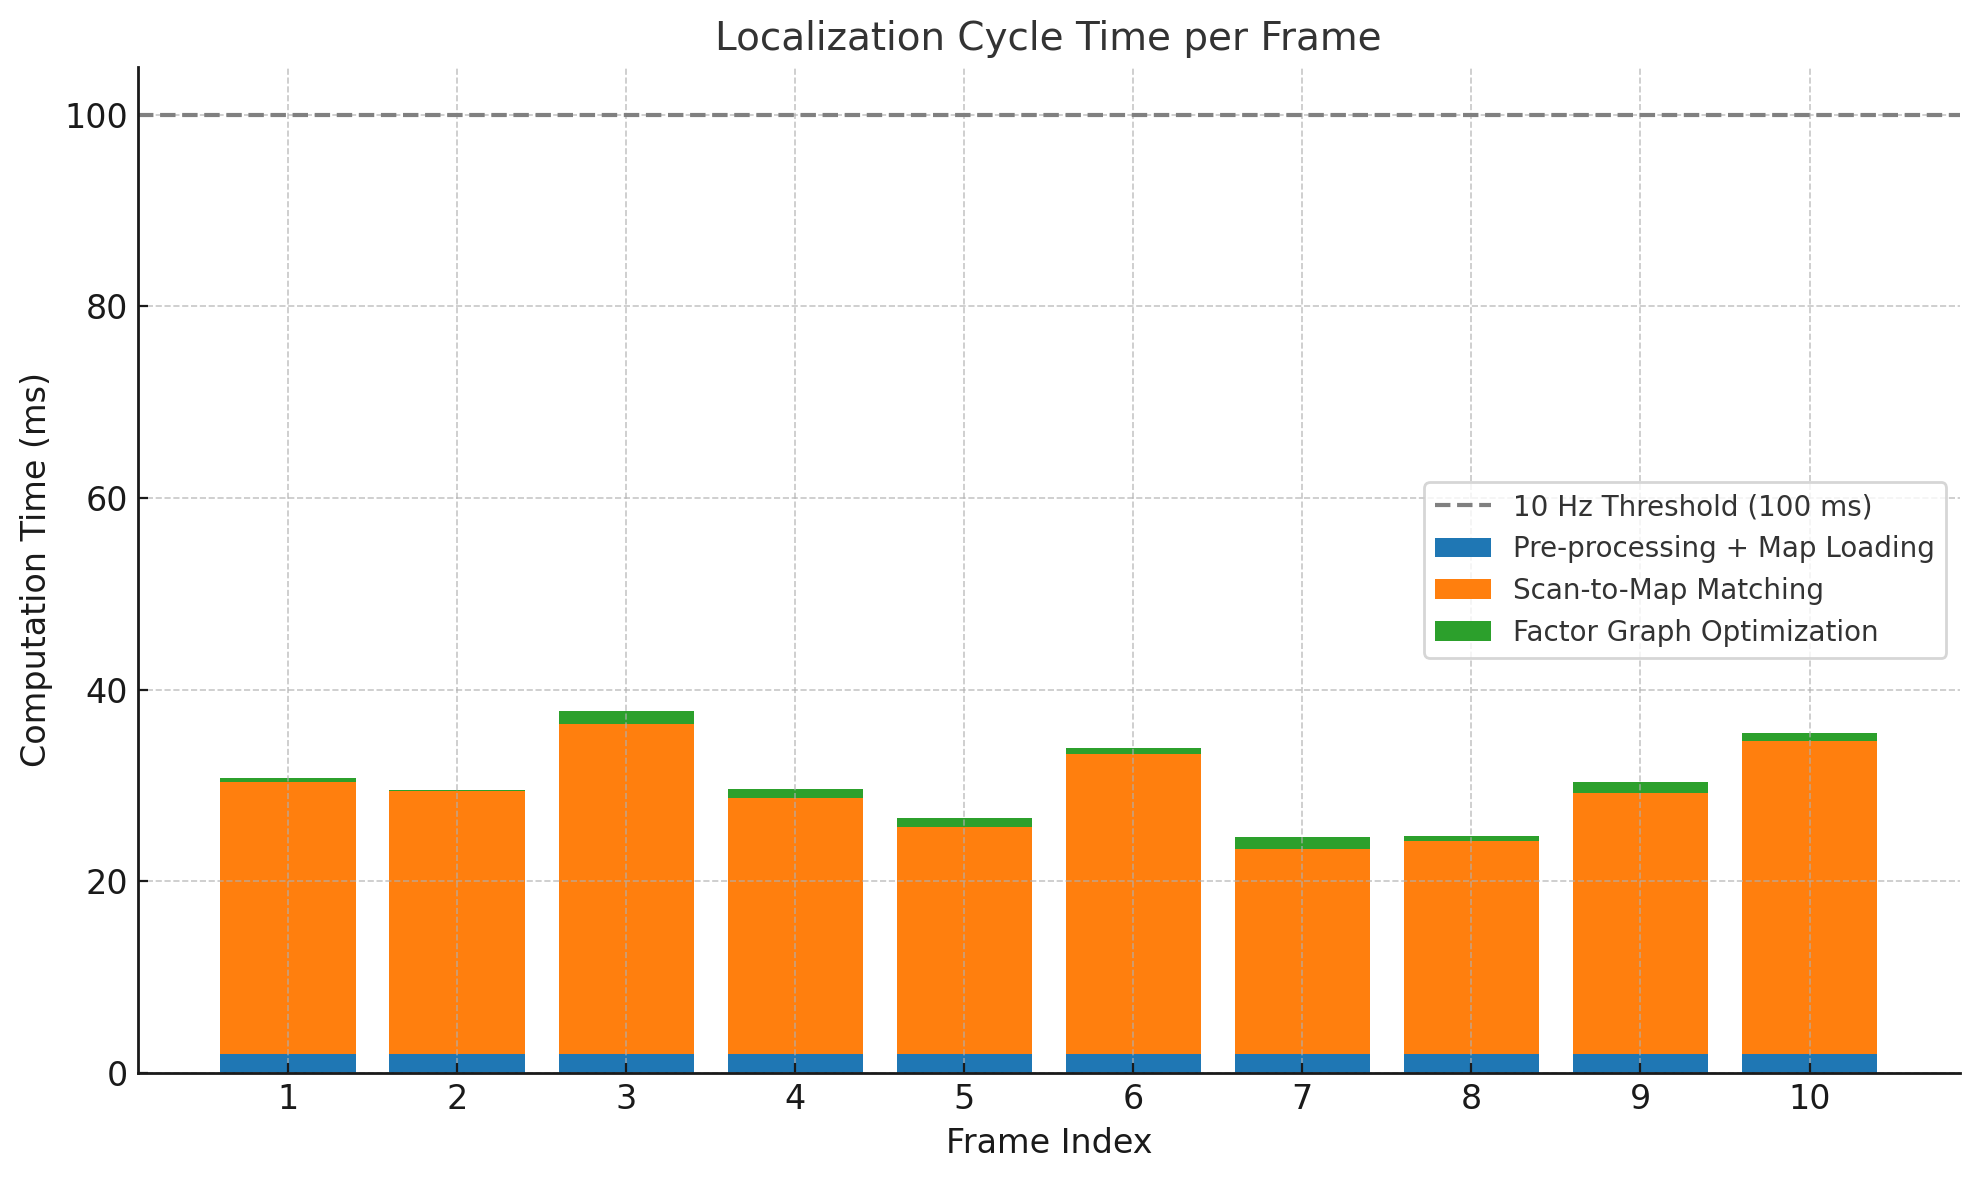
\includegraphics[width=\linewidth ,height=\linewidth]{images/localization_cycle.png}
		\caption{Computation time breakdown per frame (stacked components).}
		\label{fig:computation_summary}
	\end{subfigure}
	\caption{Computation characteristics of the proposed localization system: Sliding-window optimization scalability and real-time frame-wise timing breakdown.}
	\label{fig:computation_summary}
\end{figure}


Considering a high-frequency LiDAR-inertial odometry (LIO) stream and periodic map-matching updates, we compare a sliding-window factor-graph optimizer against a full-batch solver. By restricting the graph to the most recent 5–50 seconds of data,as shown in Figure~\ref{fig:sliding_vs_batch} the sliding-window approach maintains nearly constant solve times under 1 ms per update regardless of localization duration. In contrast, the full-batch solver’s complexity grows superlinearly as more keyframes accumulate, eventually fail in real‐time as the numer of nodes increase.

Figure~\ref{fig:computation_summary} further breaks down the per-frame latency of the proposed system. With point-cloud pre-processing and map loading taking ~2 ms, scan-to-map matching ~25 ms, and factor-graph optimization ~1 ms, the total remains below 35 ms. This comfortably satisfies the real-time 10 Hz requirement (100 ms), achieving ~36 Hz processing frequency.

\subsection{ Extended Evaluation Under Challenging Conditions}


\subsubsection{Impact of Dynamic Object Removal on Registration Performance}

In this evaluation, we assess the impact of incorporating dynamic object removal into the localization pipeline.Example of  detected 3D bounding boxes and the corresponding retained point cloud after dynamic object removal are illustrated in Figure~\ref{fig:dynamic-object-removal}.The objective is to analyze how removing transient objects from LiDAR scans influences registration accuracy, localization robustness, and computational efficiency. Key performance indicators include registration convergence rate, average iteration count and  execution time are evaluated.

\begin{figure}[H]
\centering
\begin{subfigure}[t]{0.47\textwidth}
	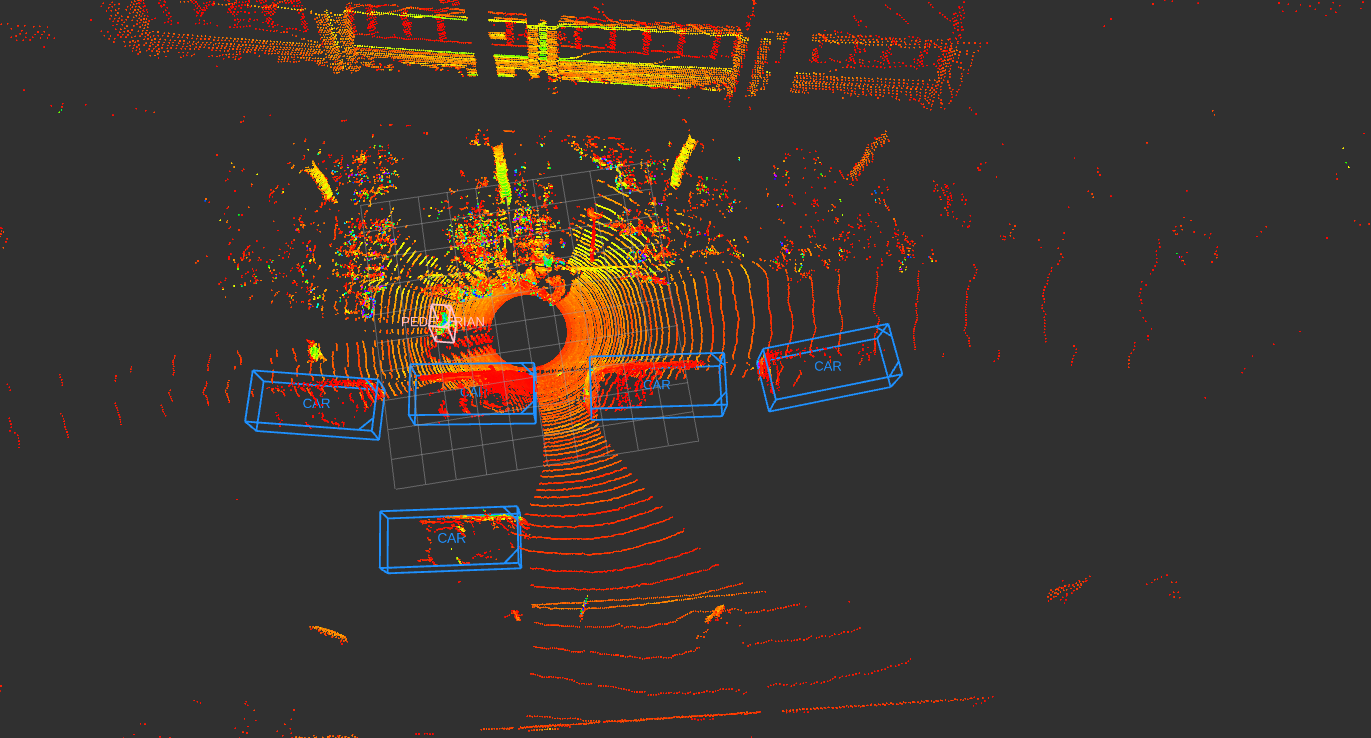
\includegraphics[width=\linewidth]{images/object_detection.png}
	\caption{3D bounding box of detected dynamic objects }
	\label{fig:3d-box-dynamic-object}
\end{subfigure}
\hfill
\begin{subfigure}[t]{0.47\textwidth}
	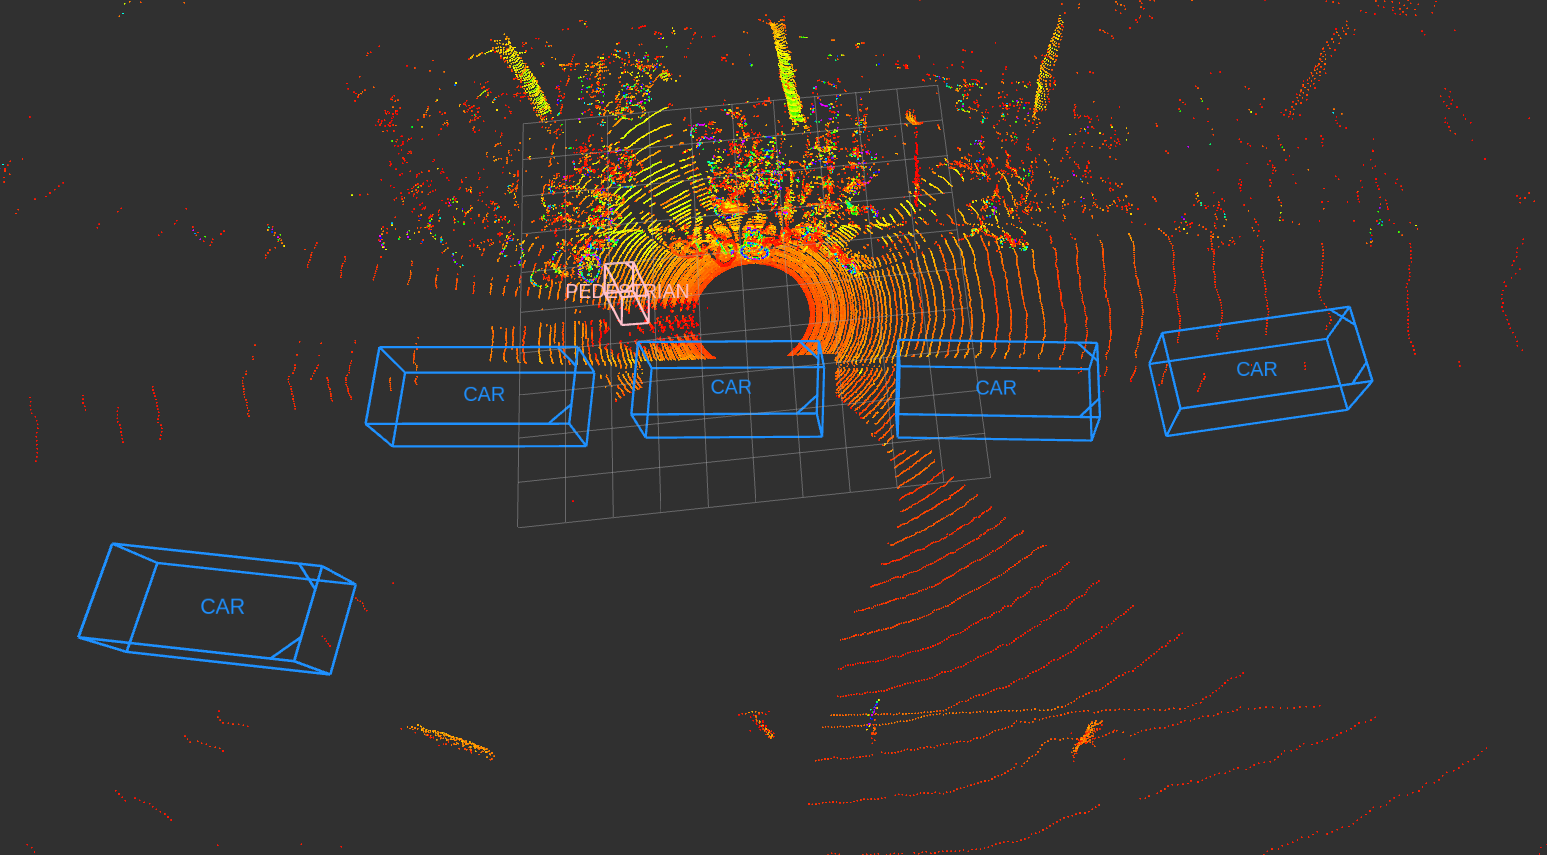
\includegraphics[width=\linewidth]{images/object_detection_remove.png}
	\caption{ Point-cloud retained after removing points with 3d bounding box.
	}
	\label{fig:3d-box-dynamic-object-removal}
\end{subfigure}
\caption[Detecting and removing dynamic objects from 3d LIDAR point-cloud]{Detecting and removing dynamic objects from 3d LIDAR point-cloud.}
\label{fig:dynamic-object-removal}
\end{figure}

\begin{table}[H]
	\centering
	\renewcommand{\arraystretch}{0.4}
	\setlength{\tabcolsep}{10pt}
	\caption{Comparison of Point-cloud Registration Metrics Before and After Dynamic Object Removal}
	\label{tab:dynamic_removal_stats}
	\begin{tabular}{@{}lccc@{}}
		\toprule
		\textbf{Metric} & \textbf{Without Removal} & \textbf{With Removal} & \textbf{Improvement} \\
		\midrule
		Avg. Registration Iterations & 19 & 12  & ↓ 7 \\
		Avg. Execution Time (ms)     & 14.41 & 9.73  & ↓ 4.68 \\
		Registration Failures        & 7     & 2     & ↓ 5 \\
		\bottomrule
	\end{tabular}
\end{table}

\begin{figure}[H]
	\centering
	\begin{subfigure}[t]{0.45\textwidth}
		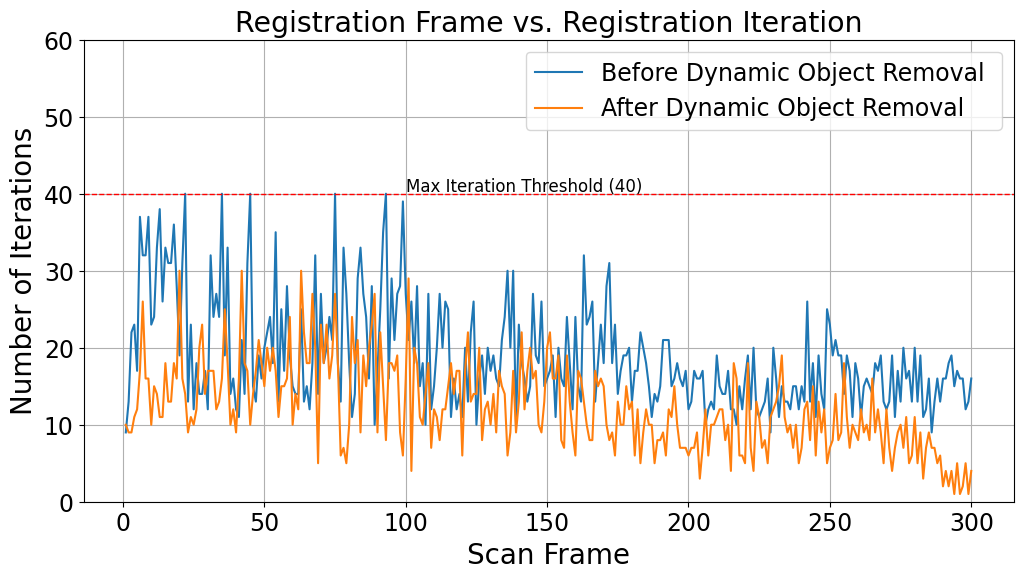
\includegraphics[width=\linewidth]{images/registration_iter_com.png}
		\caption{Registration iterations required per scan frame.}
		\label{fig:reg_iter}
	\end{subfigure}
	\hfill
	\begin{subfigure}[t]{0.45\textwidth}
		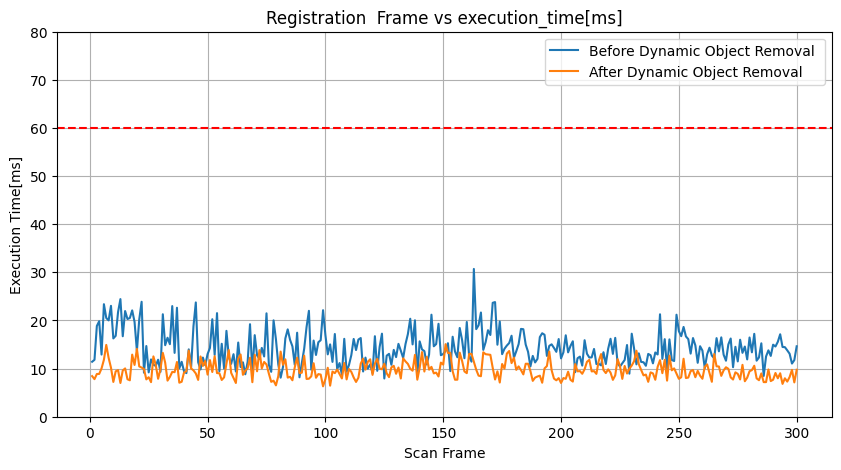
\includegraphics[width=\linewidth]{images/registration_exectime_com.png}
		\caption{Registration Execution time per frame.}
		\label{fig:reg_time}
	\end{subfigure}
	\hfill
	\begin{subfigure}[t]{0.45\textwidth}
		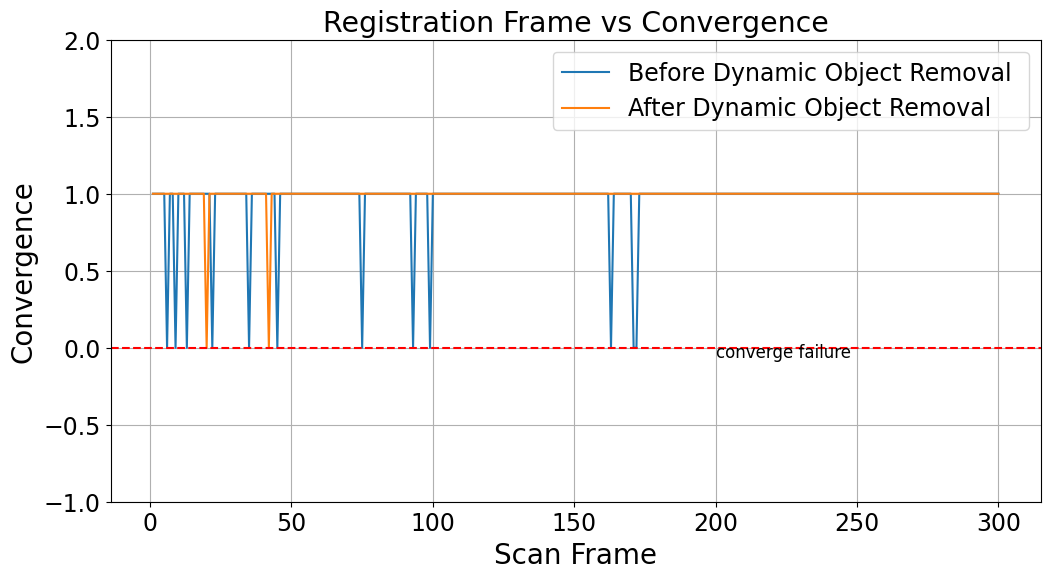
\includegraphics[width=\linewidth]{images/registration_conver_comp.png}
		 \caption{Convergence status (1 = success, 0 = failure) across frames.}
		\label{fig:reg_converge}
	\end{subfigure}
	\caption[Point-cloud Registration Performance with and without Dynamic Object Removal]{\textbf{Registration performance before and after dynamic object removal.} Each subplot shows the impact of removing dynamic objects on and iteration count (a) , execution time (b), and convergence (c). Across 300 frames, the system becomes more stable, efficient, and reliable after filtering out dynamic elements from the scan.}
	\label{fig:registration_metrics_comparison}
\end{figure}


The point-cloud registration performance was evaluated across 300 scan frames , selected based on a high number of detected dynamic objects. As summarized in Table~\ref{tab:dynamic_removal_stats}, filtering dynamic objects results  reduction in average registration iterations (from 19 to 12) and execution time (from 14.41 ms to 9.73 ms). Additionally, the number of convergence failures dropped from 7 to 2. The performance plots in Figure~\ref{fig:registration_metrics_comparison} further illustrate this trend. Dynamic object removal improves stability and efficiency by eliminating noisy inputs that otherwise increase iteration count, processing time, or lead to failed alignments.


Table~\ref{tab:dynamic_object_runtime_pipeline_comparison} presents the computational overhead introduced by integrating dynamic object detection and filtering into the localization pipeline. While this module enhances registration robustness and accuracy, it incurs additional processing time. Specifically, the 3D object detection step (using ONNX inference) adds approximately 31 ms, and the point cloud filtering (using a CropBox filter) adds another 8 ms per frame. Although the registration and optimization stage benefits from a reduction in processing time from 15 ms to 10 ms the overall per-frame runtime increases from 15 ms (without removal) to 49 ms (with removal), resulting in a net overhead of 34 ms. Despite this increase, the system remains within acceptable real-time performance bounds for medium-speed mobile robotics applications.


\begin{table}[H]
	\centering
	\renewcommand{\arraystretch}{0.3}
	\setlength{\tabcolsep}{3pt}
	\caption{Per-frame runtime analysis with and without dynamic object removal.}
	\label{tab:dynamic_object_runtime_pipeline_comparison}
	\begin{tabular}{lccc}
		\toprule
		\textbf{Component} & \textbf{Without Removal (ms)} & \textbf{With Removal (ms)} & \textbf{Overhead(ms)} \\
		\midrule
		Object Detection         & —     & 31.0  & +31.0 \\
		Point Cloud Filtering    & —     & 8.0   & +8.0 \\
		Registration and other            & 15.0  & 10.0   & ↓ 5 \\
		\midrule
		\textbf{Total}           & 15.0  & 49.0  & +34.0 \\
		\bottomrule
	\end{tabular}
\end{table}



\subsubsection{Localization on Map Side Feature Sparse Environment}

Map-side feature-sparse environments refer to areas where the current LiDAR observations contain few or no correspondences in the prebuilt map. This situation typically arises at the boundaries of a mapped area, in unmapped zones, or at transitions between separately built or merged submaps. In such regions, the prior map lacks persistent geometric features required for reliable scan-to-map registration, resulting in degraded or failed localization if scan matching is used in isolation.

\begin{figure}[H]
	\centering
	\begin{tikzpicture}		
		% Main trajectory image
		\node[anchor=south west, inner sep=0] (main) at (0,0)
		{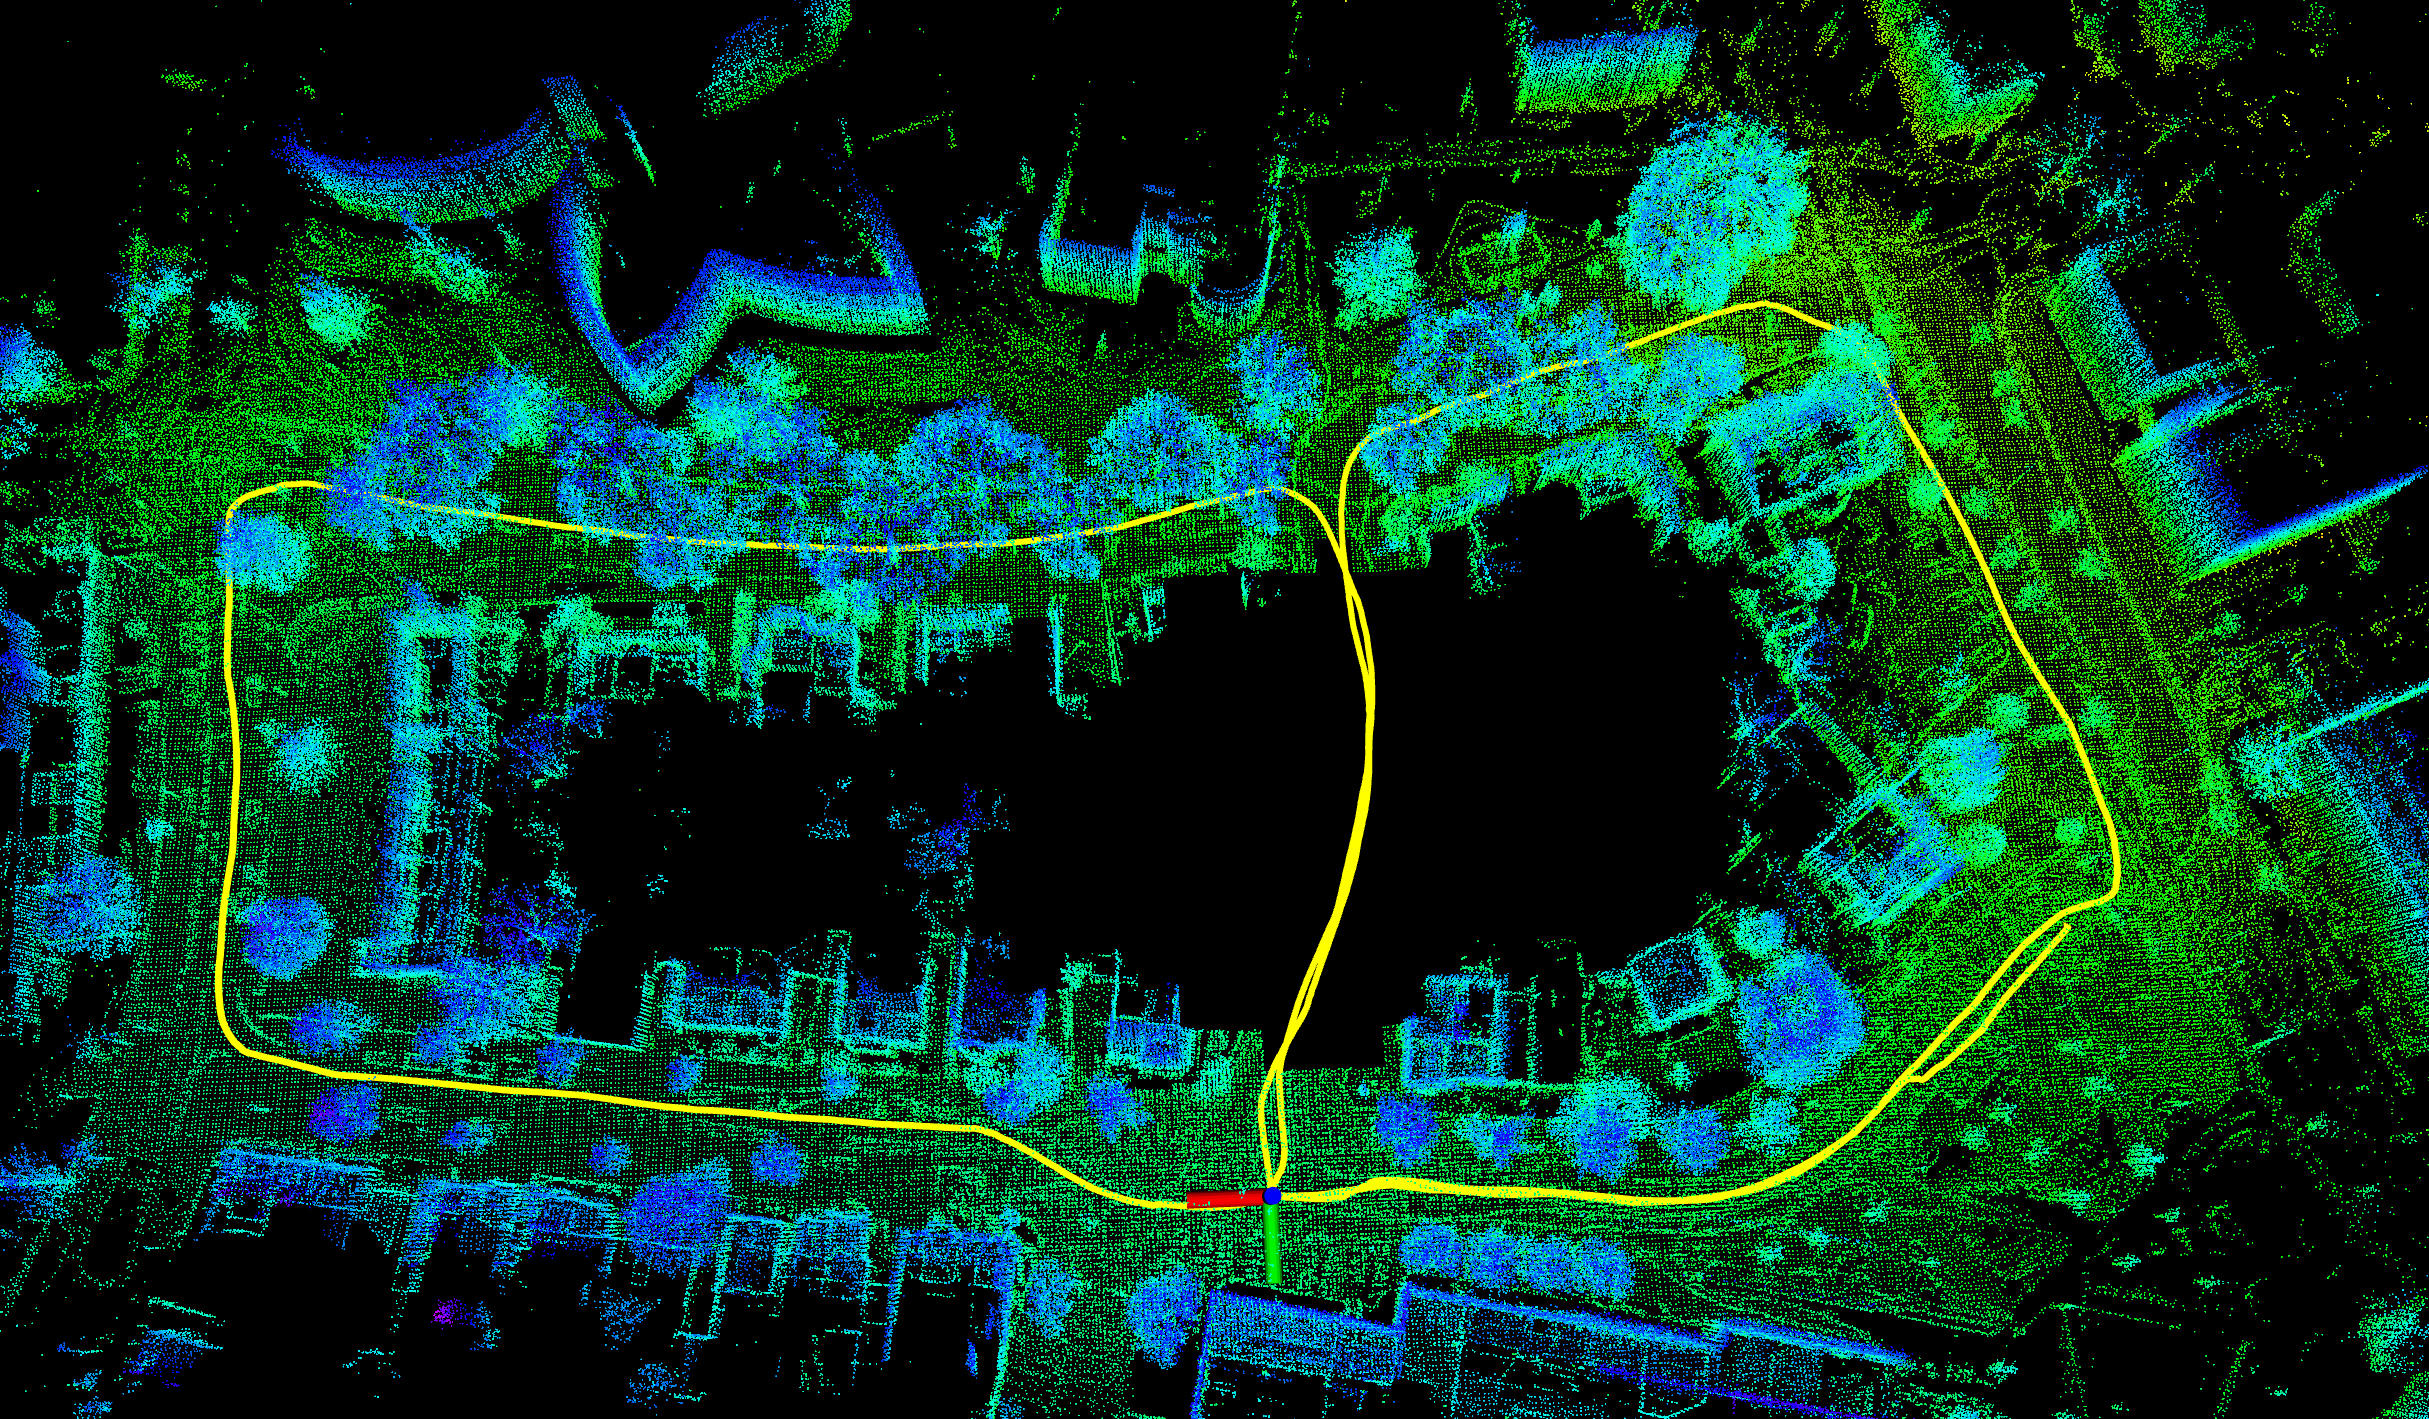
\includegraphics[width=0.6\textwidth]{images/unmapped_zone2.png}};
		% Coordinate system normalized to the image
		\begin{scope}[x={(main.south east)}, y={(main.north west)}]
			% Red dashed rectangle for zoom box (adjust coordinates!)
			\draw[red, line width=1.5pt, dash pattern=on 4pt off 2pt] (0.48, 0.25) rectangle (0.59, 0.58);
			% Red arrow from zoom box o tzoomed-in image
			\draw[->, red, thick] (0.95, 0.55) -- (0.97, 0.57);
			% Add label above the rectangle
			\node[white] at (0.535, 0.41) {transition zone: 70m};
		\end{scope}
		
		
		
	\end{tikzpicture}
	
	\caption[]%
	{\textbf{	Localization in transition zone.} The robot enters a transition region (highlighted in red) where LiDAR scan matching fails due to the absence of stable features in the prebuilt map
	}
	\label{fig:unmapped-zone}
\end{figure}

In this scenario, the robot traverses an approximately 70-meter-long transition sub-street connecting two main streets, which includes partially mapped and unmapped segments. As shown in Figure~\ref{fig:unmapped-zone}, this zone is highlighted in red. This path was repeated twice to validate consistency. The NDT-based scan matching frequently failed within this zone due to the lack of map overlap, as reflected in the significant error spikes shown in Figure~\ref{fig:ape-error-unmapped-ndt}, \ref{fig:ape-error-trajectory-unmapped-proposed}. However, the proposed fusion pipeline maintained stable localization throughout the traversal shown in Figure~\ref{fig:ape-error-unmapped-proposed}.

A comparison of APE statistics is summarized in Table~\ref{tab:ape-unmapped-comparison}. Notably, the maximum APE for NDT Scan Matching reached 2.178 meters, whereas the proposed fusion method limited the maximum error to 0.455 meters. The Root Mean Square Error (RMSE) also showed a significant reduction, from 0.295 meters in NDT to 0.095 meters in the fusion approach. These results underscore the robustness of the proposed method in feature-deprived environments.


For context, under standard conditions specifically, Saxion Sequence 1 APE statistics is summarized in Table ~\ref{tab:ape_rot_saxion_seq1}, which was conducted in a fully mapped environment the proposed fusion method achieved a maximum APE of 0.395 meters and an RMSE of 0.067 meters. This comparison underscores the robustness of the fusion approach, demonstrating its ability to maintain localization accuracy even in challenging, feature-sparse environments.

\begin{figure}[H]
	\centering
	\begin{subfigure}[t]{0.49\textwidth}
		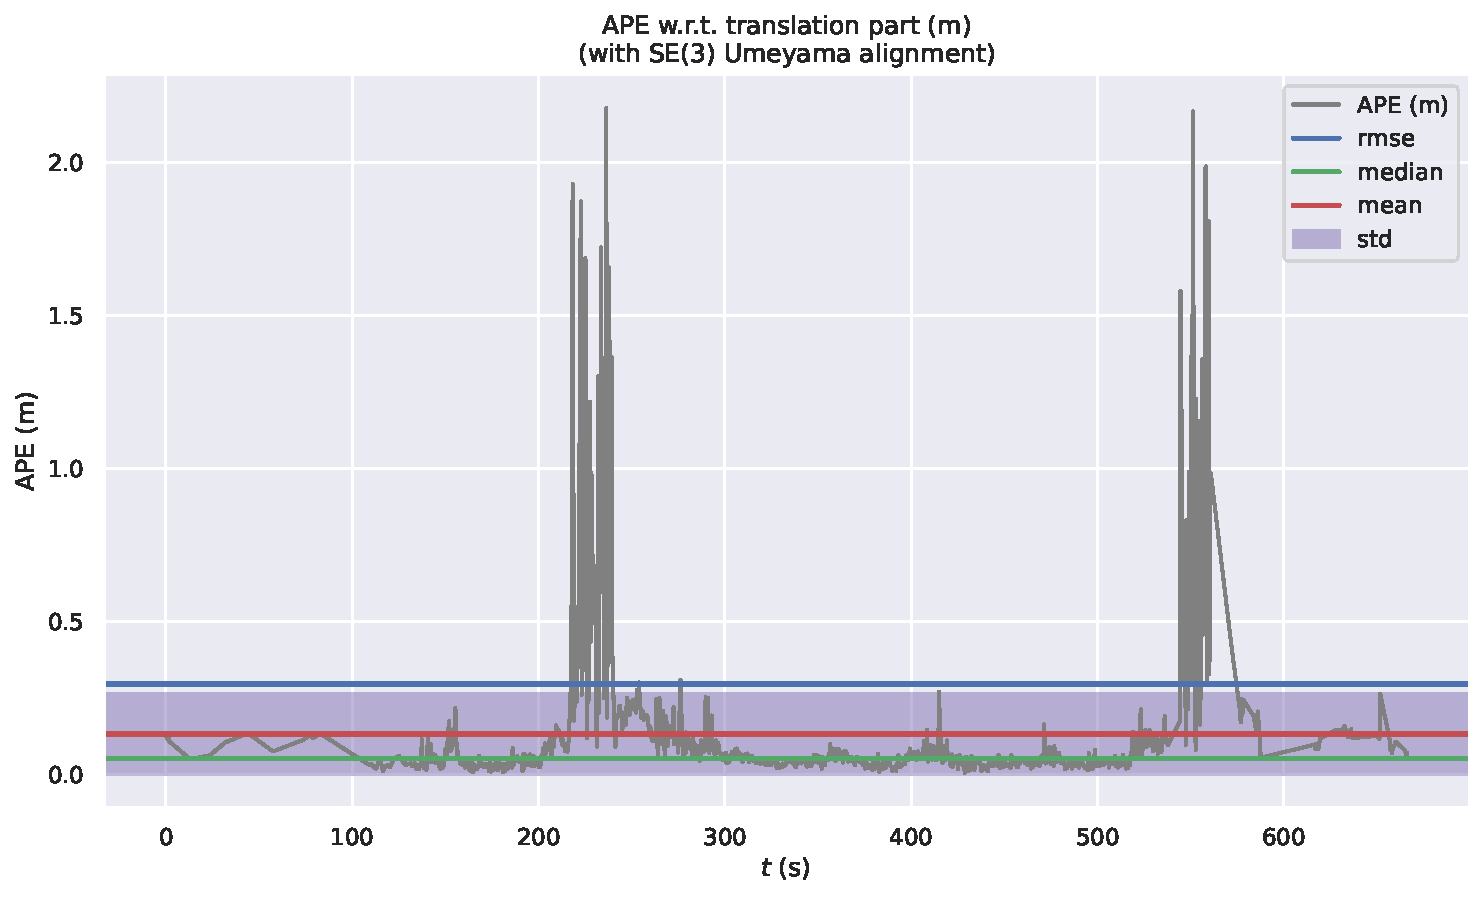
\includegraphics[width=\linewidth]{images/unmappedzone_error_ndt2.pdf}
		\caption{ NDT Scan Matching  APE - translation part  }
		\label{fig:ape-error-unmapped-ndt}
	\end{subfigure}
	\hfill
	\begin{subfigure}[t]{0.49\textwidth}
		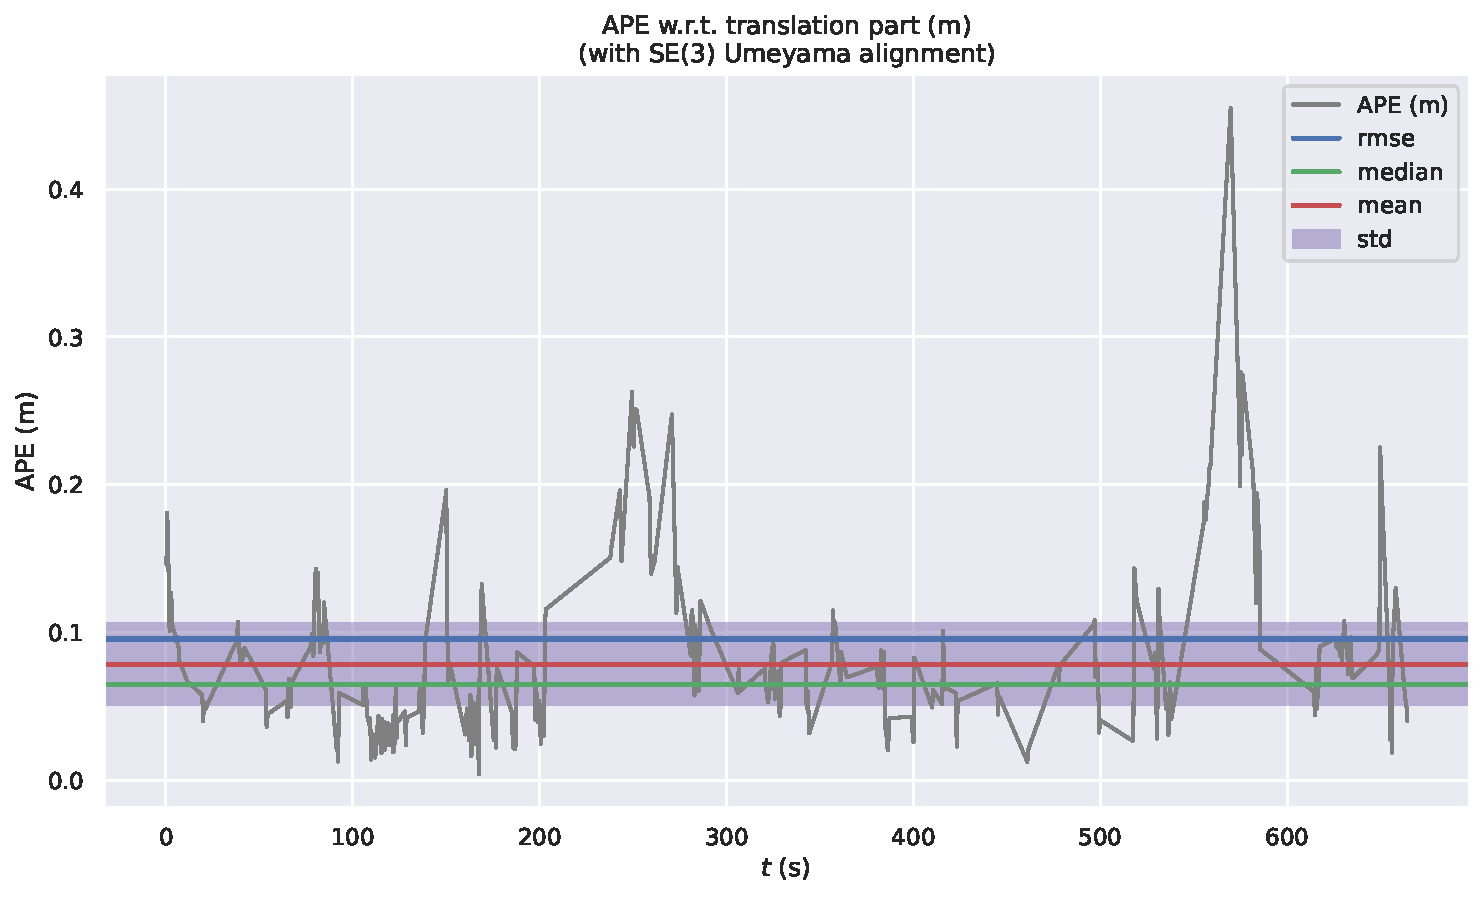
\includegraphics[width=\linewidth]{images/unmapped_zone_error_fused.pdf}
		\caption{ Proposed - translational part
		}
		\label{fig:ape-error-unmapped-proposed}
	\end{subfigure}
    \begin{subfigure}[t]{0.49\textwidth}
    	\includegraphics[page=2 ,width=\linewidth]{images/unmappedzone_error_ndt2.pdf}
    	\caption{ NDT Scan Matching APE Trajectory  - translation part.
    	}
    	\label{fig:ape-error-trajectory-unmapped-proposed}
    \end{subfigure}
	\caption[Error compression  localization in transition zone]{
	\textbf{Error compression  localization in transition zone} The APE for NDT scan matching(a) , Proposed(fusion)(b) and NDT APE trajectory(c)}
	\label{fig:ape-error-unmapped}
\end{figure}

\begin{table}[H]
	\centering
	\caption{Absolute Pose Error (APE) Statistics in Transition Corridor}
	\label{tab:ape-unmapped-comparison}
	\begin{tabular}{lcccc}
		\toprule
		\textbf{Method} & \textbf{Max APE (m)} & \textbf{Mean APE (m)} & \textbf{RMSE (m)} & \textbf{Std Dev (m)} \\
		\midrule
		Proposed Fusion   &\textbf{ 0.455} & \textbf{0.078} & \textbf{0.095} &\textbf{ 0.054} \\
		NDT Scan Matching & 2.178 & 0.131 & 0.295 & 0.264 \\
		FAST-LIO2   & 7.59 & 1.456  & 2.197 & 1.645 \\
		
		
		\bottomrule
	\end{tabular}
{\footnotesize \textit{Note:} Bold values indicate the best performance across each metric.}
\end{table}


\subsubsection{Localization Under Fog Degradation with a Recent Map}

We tested the localization pipeline on the \textbf{Saxion Sequence 1} using a one-month-old prebuilt map and simulated fog at three visibility levels: \textit{Mild (100~m)}, \textit{Moderate (60~m)}, and \textit{Severe (30~m)} see Table~\ref{tab:noise_levels}. Figure~\ref{fig:fog_visualization} illustrates fog-induced degradation effects such as point dropouts, false near-field returns, and spatial clutter. The resulting {Absolute Pose Error (APE)} was compared against a baseline under clear conditions.


Under Mild and Moderate fog Table~\ref{tab:ape_fog_translation}, the proposed fusion and NDT only methods show limited degradation compared to the baseline (Table~\ref{tab:ape_rot_saxion_seq1}).APE increses to 0..10-0.28 m , with occasional peaks over 1.4 m, but RMSE remains stable, confirms the robustness of NDT under moderate visibility loses.In contrast,FAST-LIO2 drifts significantly, with higher mean RMSE values, indicating its sensitivity to fog when operating without map-based correction.

Under Severe fog (visibility 30~m), all methods show significant degradation. The {NDT scan matcher becomes unstable} and fails to converge consistently due to severe point dropout and noise. {Fast-LIO also exhibits large drift}, and the combined effect causes the {fusion pipeline to fail repeatedly}, unable to maintain consistent localization beyond a short distance.
 
\begin{figure}[H]
	\centering
	\begin{subfigure}[t]{0.46\textwidth}
		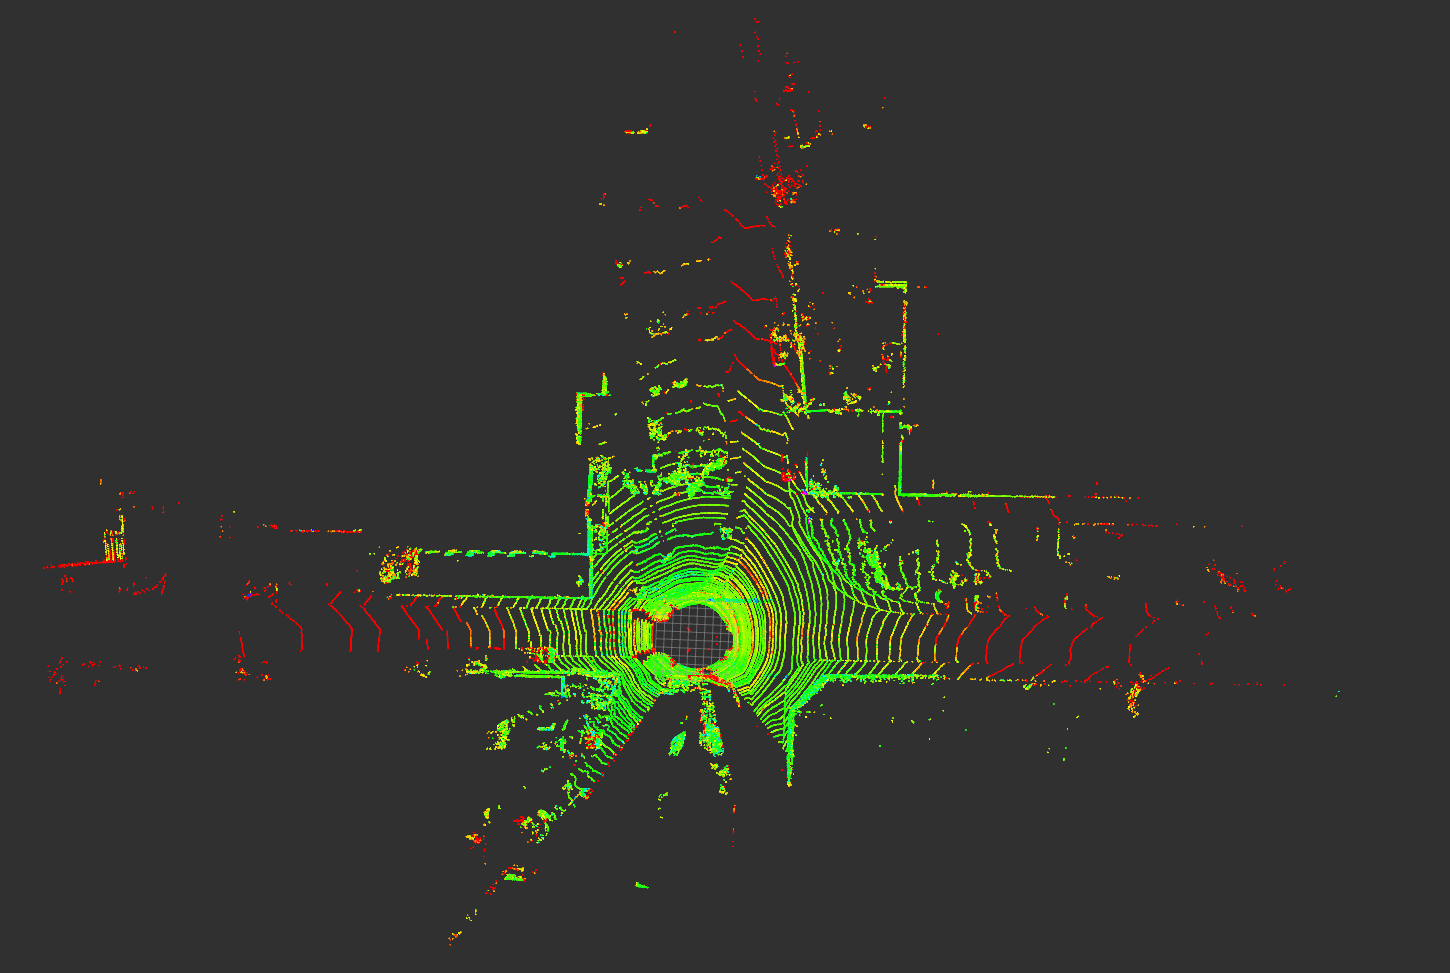
\includegraphics[ height=3.5cm , width=\linewidth]{images/original_pointcloud.png}
		\caption{ Original Point-cloud }
		\label{fig:original-noise-level-pointcloud}
	\end{subfigure}
	\hfill
	\begin{subfigure}[t]{0.46\textwidth}
		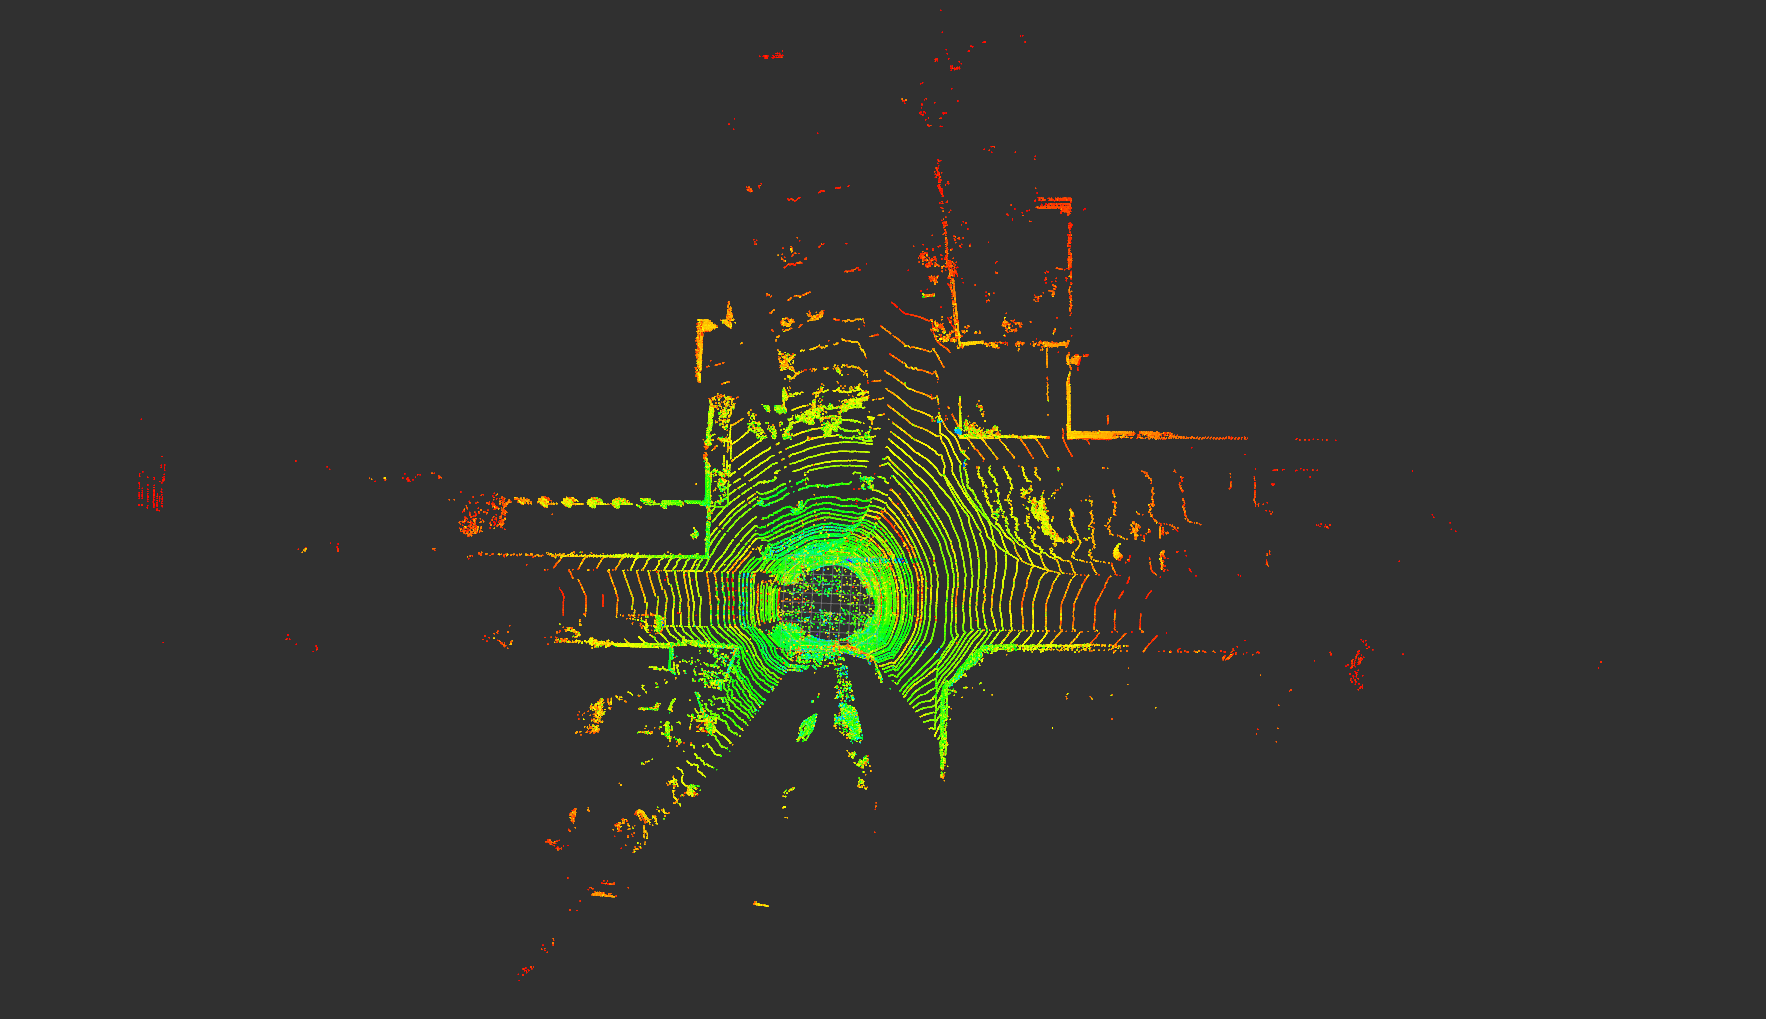
\includegraphics[height=3.5cm , width=\linewidth]{images/level1_noisea.png}
		\caption{ Mild noise level added point-cloud
		}
		\label{fig:mild-noise-level-pointcloud}
	\end{subfigure}
	\hfill
	\begin{subfigure}[t]{0.46\textwidth}
		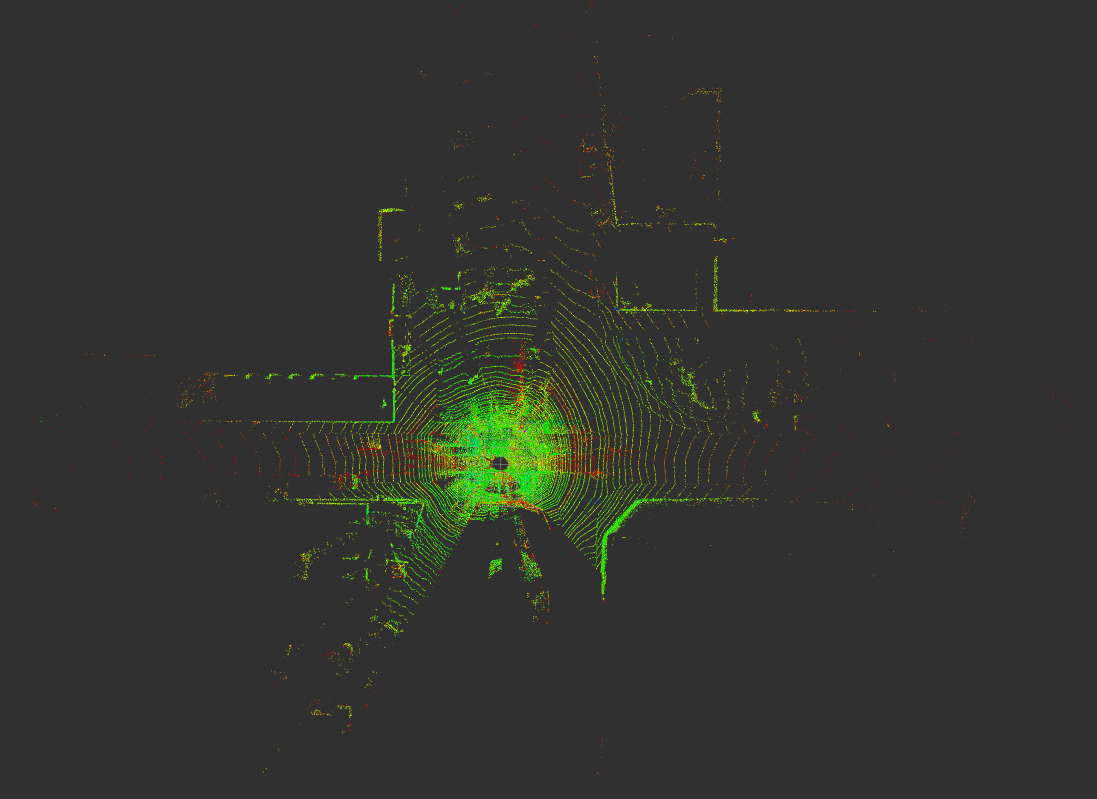
\includegraphics[height=3.5cm , width=\linewidth]{images/noise/15.png}
		\caption{ Moderate noise level added point-cloud
		}
		\label{fig:severe-noise-level-pointcloud}
	\end{subfigure}
	\hfill
	\begin{subfigure}[t]{0.46\textwidth}
		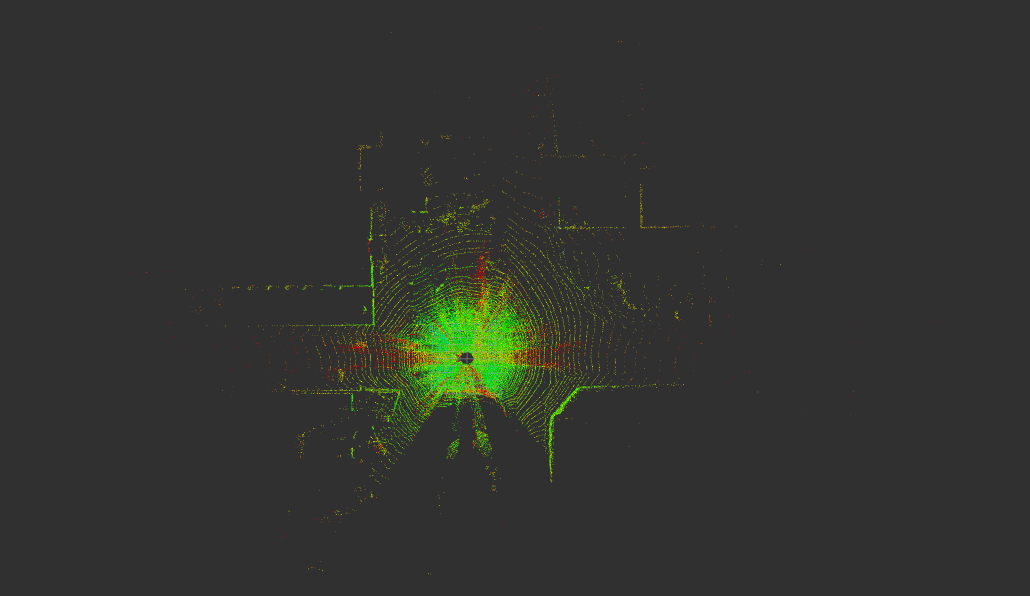
\includegraphics[height=3.5cm , width=\linewidth]{images/noise/14.png}
		\caption{ Severe noise level added point-cloud
		}
		\label{fig:mild-noise-level-pointcloud}
	\end{subfigure}

		
	\caption{Point‐cloud snapshots under increasing composite geometric noise levels: (a) Original scan; (b) Mild noise; (c) Moderate noise; (d) Severe noise.}
	
	\label{fig:fog_visualization}
\end{figure}




\begin{table}[H]
	\centering
	\caption{Translation error (APE) statistics under Severe and Moderate  fog visibility}
	\label{tab:ape_fog_translation}
	\begin{tabular}{l l c c c c c}
		\toprule
		\textbf{Condition} & \textbf{Method} & \textbf{Max} & \textbf{Mean} & \textbf{Min} & \textbf{RMSE} & \textbf{Std Dev} \\
		\midrule
		
		\multirow{3}{*}{Mild} 
		& Proposed     & 0.3682 & 0.1238 & 0.0250 & 0.1356 & 0.0583 \\
		& NDT          & 0.4089 & 0.1474 & 0.0164 & 0.1585 & 0.0581 \\
		& Fast-LIO     & 12.0253 & 4.2643 & 0.581 & 5.7521 & 3.2145 \\
		
		\midrule
		
		\multirow{3}{*}{Moderate} 
		& Proposed     & 0.3792 & 0.1326 & 0.0092 & 0.1452 & 0.0593 \\
		& NDT          & 1.3442 & 0.1712 & 0.0193 & 0.2178 & 0.1346 \\
		& Fast-LIO     & 17.7823 & 6.2.3521 & 0.0610 & 12.9345 & 5.3614 \\
		
		\bottomrule
	\end{tabular}
\end{table}





